\chapter{Cetacean Detection Using Deep Learning}\label{ch:cetDet}

When building any large-scale project, it is important to break the task down into various subcomponents. This Chapter examines one such subcomponent utilised in the development of an automatic photo-id system, the cetacean detector. This component takes images captured during photo-id surveys and locates regions of interest (RoIs) - defined as areas in which a dorsal fin breaches the waterline. This Chapter will discuss the requirements a detector must meet, as well as its training and hyperparameter optimisation. 

\section{Requirements of a Cetacean Detector}\label{ch:cetDet,sec:requirements}

Before a system for automatic cetacean detection can be developed, it is important to first define the problem and understand the requirements of the system. The overall aim of the detector is to be able to take large-scale images as input, fed in one at a time, and process them in order to locate RoIs. This detector will only be required to identify one object class, dolphins. These detected regions can then be passed further down the system pipeline for photo-identification. 

 As such this detector can be considered a coarse-grain task, and at first glance may seem somewhat trivial. However due to both the nature of the environment in which the RoIs must be detected, and the technical requirements the system must perform under, this is actually a complex problem. 
 
 \subsection{Environmental Requirements}\label{ch:cetDet,sec:requirements,sub:environmental}
 
 Firstly the area in which this system is to be deployed, open water, is susceptible to adverse weather conditions such as high winds. This in turn leads to sub-optimal conditions for detection which the system must be capable of handling, most notably high amounts of sea swell. Further to this, cetaceans are communal and travel in pods. An example of this behaviour can be seen in Figure \ref{fig:pod-eg}. Thus, the system must be capable of differentiating between overlapping individuals. Even if not all of the overlapping individuals are suitable for identification downstream, the system must still be able to separate them into individual detections to prevent misclassification.
 
 \begin{figure}
 	\begin{center}
 		\includegraphics[scale=0.06]{Chapter3/figs/dolphins-in-pod-example.JPG}
 	\end{center}
 	\caption{Some cetaceans, such as bottlenose dolphins, travel in pods. The developed detection system must be capable of splitting this pod into individual animals to be passed to the identifier.
 	}
 	\label{fig:pod-eg}
 \end{figure}

 Next, the detector must be capable of differentiating between dolphin fins and waves. Again this might sound trivial, but thousands of years of evolution have resulted in fins and waves looking extremely similar to the untrained (artificial) eye. Especially from a distance and in choppy waters, fins and waves often have extremely similar shape and structure. Furthermore, the animal's bodies are also similarly coloured to their surroundings. These adaptations allow the animals to be better protected and camouflaged in their environment, but can cause issues with detection systems. This becomes apparent when thinking about how CNNs \textit{see}. As described in Chapter \ref{ch:Background,sec:DLforCV}, CNNs see input images as a matrix of pixel values. When training an object detection system the CNN is told which parts of this matrix are related to a class, any without a class label are considered background. If fins and areas of background contain similar pixel values, and these pixel values are clustered in similar ways, this can result in issues when training a model to detect instances of a class without misclassifying the background. 
 
 Another important requirement is for the detector to be able to handle objects of varying size, shape, direction, and angle of approach. When working in an open water environment with live animals, there is no guarantee how the animal will approach the camera, and thus the detector must be generalisable enough to handle this. 
 
 Furthermore how the animals breach the water is also extremely variable. Breachings may occur in any direction relative to the boat and the animal could itself be travelling in a different cardinality. The ideal scenario in this case would be for a breaching to occur either directly East or West of the boat (off the port or starboard side respectively) with the animal travelling perpendicular as this provides the best chance capture markings - however this rarely occurs. For example, a breaching may occur off the port-side of the bow (approx North West relative to the boat), but the animal may be travelling in a South-Easterly direction. These approaches greatly change the look of the fin, although they may still contain identifiable markings. The detector should be able to detect these fins and pass them along for identification. An example of this can be seen in Figure \ref{fig:angle-eg}, which also shows how distance from the vessel can change the camera's view of the dorsal. 
 
   \begin{figure}
 	\begin{center}
 		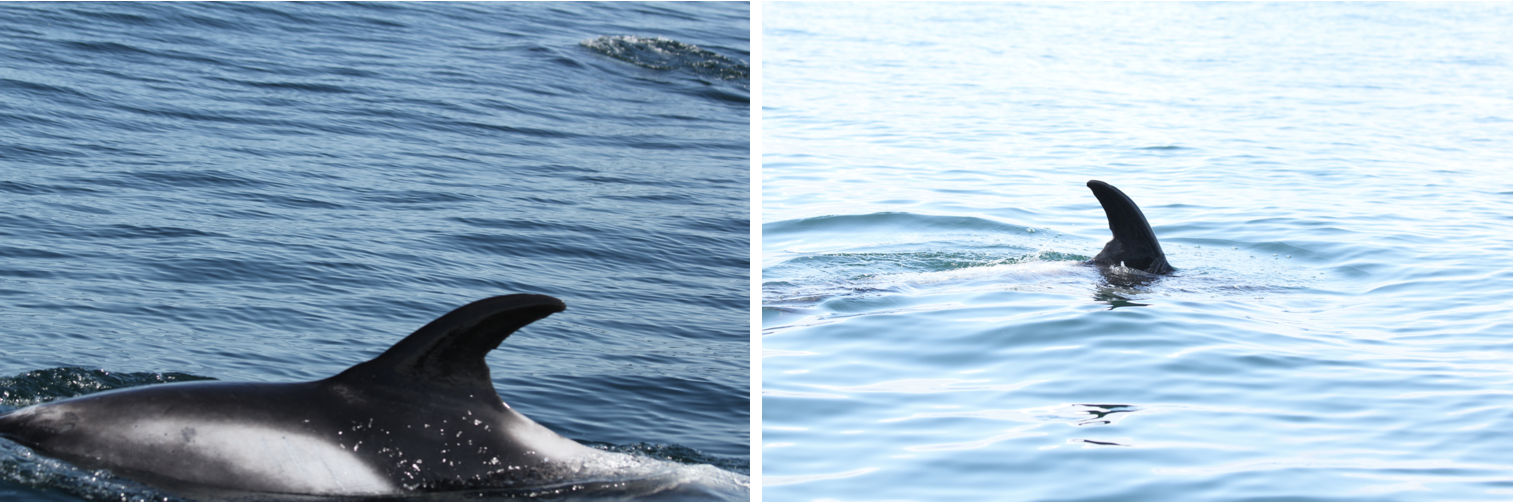
\includegraphics[scale=0.6]{Chapter3/figs/angle-size-example.png}
 	\end{center}
 	\caption{Two images of the same individual taken from different angles of approach, directions of travel, and distances from the vessel. Note how this changes the make-up of the dorsal fin but keeps the identifying notch visible. 
 	}
 	\label{fig:angle-eg}
 \end{figure}
 
 As mentioned previously, weather conditions can also greatly affect how a dorsal fin is captured by a camera. However in photo-id surveys there are only two conditions that need to be worried about; swell and lighting. This is due to most research groups limiting travel in rough seas for safety reasons. With regards to Newcastle University's Marine MEGAfauna Lab, this limit is a sea state less than 3 on the Beaufort scale \cite{world_meteorologicial_society_beaufort_1970}. As such, a mild amount of swell and splash can be expected which the detector should be capable of handling. Lighting conditions are not considered in the Beaufort scale, but for operational reasons the vast majority of photo-id surveys take place during daylight hours. This can lead to large amounts of glare in images, especially on clear days. The detector should be invariant to these conditions. 
 
 \subsection{Technical Requirements}\label{ch:cetDet,sec:requirements,sub:technical}
 
On top of being able to handle a variety of environmental factors, there are also some technical requirements that the detector must meet. With all deep learning based computer vision approaches, there is often a trade off that must be made between speed and accuracy. In most cases, these are inversely proportional to each other; the faster a system is required to perform, the lower an accuracy you must be willing to tolerate - Huang \textit{et al.} discuss this in greater detail \cite{huang_speedaccuracy_2017}. Thanks to the pace of research in this area, 2020 saw the release of detection architectures which can perform operations in real-time such as EfficientDet \cite{tan_efficientdet_2020} and YOLOv4 \cite{bochkovskiy_yolov4_2020}. Current accuracies on benchmark datasets using these real-time architectures are still a long way off their non-real-time competitors however, and accuracies would drop further on custom non-benchmark tasks such as cetacean detection. 
 
 Because this trade off must be made, before deploying a deep learning model it is important to decide where the system will be utilised. As photo-id surveys are performed on small vessels such as RIBs, space is severely limited on board. Because of this, it is not appropriate to add additional hardware to the vessel to perform this analysis during the survey. Furthermore, the current methodology of cetacean researchers is to perform identification once back on land, even when utilising photo-id aides. As the system proposed in this project is intended to fit into existing procedures rather than replace them, it is appropriate for the system to also be land based rather than on the vessel. Thinking about the current procedure further, this project's proposed system could be, for example, left running overnight performing identifications whilst the researchers are asleep or during the day whilst they are on surveys. As such, there is no need for the system to operate in real time to fit in with the current workflow of cetacean researchers provided the system completes its task within a reasonable time frame. Further to this, as the output of the detection model will be passed to an identification module, it is imperative that as much noise is removed as possible during the detection. In order to do this, the accuracy of the detection must be as high as possible, furthering the case for an accurate system over a fast one.
 
 This idea of reducing as much noise as possible can be used to further narrow down the requirements of the detection system. As discussed in Section \ref{ch:Background,sec:DLforCV}, the output of detection systems can be provided in different formats. In bounding box detection systems the detected objects are described by a set of at least two pixel coordinates denoting the top-left and bottom-right extremes of the object. These detections are often more cost-effective, both from a labelling perspective requiring less person-hours to complete, and to perform computationally. Bounding box based detections are limited in their ability to remove background noise however, with only the background outside of the box removed.
 
 If we utilise pixel wise mappings however, then each pixel is given a classification. This allows the system to be more discrete with its detection, allowing for the removal of as much background as possible. Both semantic and instance segmentation methods allow the detector to utilise pixel-wise mappings to remove background noise. Pixel wise labelling is far more labour intensive and costly to produce compared to bounding box labelling, and systems capable of pixel level detections are often slower than bounding box detectors. Utilising our requirements as defined in Section \ref{ch:cetDet,sec:requirements,sub:environmental}, specifically that the detector must be capable of reducing an overlapping pod to its individual component animals, the use of pixel wise mappings at an instance level would be preferable over semantic or bounding box level detections. This requirement reveals a further trade-off the system must make. The amount of noise removed by the detector is proportional to the cost and labour needed to create data to train the system. This is discussed in more detail in Section \ref{ch:cetDet,sec:deciding,sub:boundingBoxInvestigation}.
 
 Furthermore, any system performing cetacean detection from photo-id survey data must be capable of working with large scale images. In most image based tasks where deep learning is utilised images fed to the network are downscaled, typically to sizes such as 224x224 to allow for faster training and a reduction in overall network size. Downscaling images reduces the number of pixels in the image, which by definition reduces the amount of information present as pixels values need to be pooled (one pixel needs to now display what multiple would have previously). For most detection tasks this would not be an issue, and indeed if this project was solely a cetacean detection task there would be no issues with downscaling. This detector is not stand-alone however but rather the first stage of a pipeline of networks with the end goal of photo-identification. The identification task relies on potentially minute details in the fin such as notches; any downscaling of the image at the detection stage runs the risk of removing potentially identifiable information in the fin. As such, the image must only be reduced in size once it is certain that no identifying information will be lost. As this cannot be guaranteed at the stage of detection, the detector must be capable of operating on images without resizing.
 
\section{Deciding on Architecture and Framework}\label{ch:cetDet,sec:deciding}

Based on the requirements outlined in Section \ref{ch:cetDet,sec:requirements}, it is possible to begin deciding on how the cetacean detector is to be developed. One of the most important factors in the overall approach taken in the detector's development, and ultimately the overall automatic photo-id system, would be the use of either bounding boxes or pixel-wise mappings. As mentioned previously, the use of pixel-wise mappings would allow for a greater removal of background noise, but is extremely costly and labour intensive to produce. In contrast, bounding box labels are easier and cheaper to produce but will lead to less background noise removal. 

\subsection{An Investigation into Bounding Boxes}\label{ch:cetDet,sec:deciding,sub:boundingBoxInvestigation}

Due to their relative cheapness and ease to produce, the use of bounding boxes in this project would be extremely beneficial. However, if the use of bounding boxes at this stage would hinder the accuracy of individual identification downstream, then this would outweigh the cost of pixel-wise mappings. 

As such, an investigation was undertaken to decide whether bounding boxes would be a viable option and if their use would hinder downstream identification. To begin, a small amount of data was provided by the Marine MEGAfauna Lab at Newcastle University, discussed in more detail in Section \ref{ch:cetDet,sec:initialTesting,sub:zanzibar}, which contained images captured during a previous cetacean survey. A subset of this data was manually cropped to simulate the output of a bounding box detector, an example of which can be seen in Figure \ref{fig:manual-crop-example}. This manually cropped data included some background but ensured the RoI, the dorsal fin, was centred and prominent representing an optimal output from a bounding box detector. 

\begin{figure}
	\begin{center}
		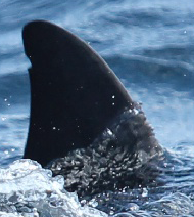
\includegraphics[scale=0.6]{Chapter3/figs/manual-crop-example.png}
	\end{center}
	\caption{An example manual crop utilised in bounding box suitability testing.
	}
	\label{fig:manual-crop-example}
\end{figure}

\subsubsection{Feature Extraction with SIFT}\label{ch:cetDet,sec:deciding,sub:boundingBoxInvestigation,subsub:SIFT}

To begin, processing of the cropped images focussed on the use of feature extractors such as Scale-Invariant Feature Transform, also known as SIFT \cite{lowe_object_1999}. As the name suggests SIFT is invariant to scale, a major advantage for use with cetacean survey data where the RoI's size may change depending on when the image of the dorsal fin breaching the water is captured. If SIFT was capable of producing feature descriptors of the dorsal fins with only partial background removal, this would show potential for individual identification where some background is present, possibly through the use of the feature descriptors.

First SIFT was performed over the entire cropped image. This proved unfruitful however, picking out very few features in areas of the image which contained the animal's dorsal fin and instead focussing on the feature heavy areas present in the sea even in images containing relatively calm water. This result indicated that further refinement was required, potentially reducing the area SIFT was allowed to explore. 

Reduction of the search space available to SIFT was achieved through the use of colour thresholding. Here, a mask was created programmatically for each image based on bounded RGB colour values found in the dorsal fins, giving an upper threshold of (14, 16, 26) and a lower threshold of (54, 51, 66). As such, SIFT would only be performed in areas of the image where pixel values fell within this range. An example result of SIFT after colour thresholding can be see in Figure \ref{fig:manual-crop-sift-colour-thresholding-example}, with coloured circles surrounding an extracted feature. As can be seen, colour thresholding helps in removing a large amount of background water from the computation. Issues arise however where areas of water are also within this thresholding. Because of this, colour thresholding before SIFT only reduces the amount of features extracted from the water, it does not remove them, which may result in misidentification downstream.

Further to this, it can be seen that SIFT is incapable of extracting relevant prominent markings from the species in the image, Indo-Pacific bottlenose dolphins (\textit{Tursiops aduncus}). For example, in Figure \ref{fig:manual-crop-example}, a notch is clearly present on the dorsal fin which is a good marker for individual identification. However, when performing SIFT on this dorsal as seen in Figure \ref{fig:manual-crop-sift-colour-thresholding-example}, note how this notch has not been detected by SIFT, which has instead detected an area above the notch which contains no identifiable information. 

\begin{figure}
	\begin{center}
		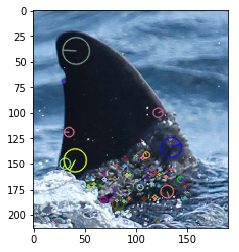
\includegraphics[scale=0.6]{Chapter3/figs/manual-crop-sift-colour-thresholding.png}
	\end{center}
	\caption{An example manual crop showing the result of SIFT feature extraction when thresholded based on RGB colour values.
	}
	\label{fig:manual-crop-sift-colour-thresholding-example}
\end{figure}

Feature extraction methods such as SIFT are also incapable of extracting other identifiable markers such as fin shape. As such, the use of SIFT was deemed improper for this use case. It is important to note here that the use of SIFT may be appropriate for cetacean species other than this project's data subjects of bottlenose and white-beaked dolphins. For example, the use of SIFT has been shown to be appropriate to aid in identification of individual Risso's dolphins by Maglietta \textit{et al} \cite{reno_sift-based_2019}.

\subsubsection{Background Removal with GrabCut}\label{ch:cetDet,sec:deciding,sub:boundingBoxInvestigation,subsub:GrabCut}

Testing the suitability of SIFT as described in Section \ref{ch:cetDet,sec:deciding,sub:boundingBoxInvestigation,subsub:SIFT} highlighted the need for complete background removal before identification would be possible with bottlenose and white-beaked dolphins. In order for bounding boxes to be a viable option in this scenario, a robust background removal process would need to be created. Further, the process would need to be capable of operating under unseen conditions in an unsupervised manner without pixel labelled data to train on. If the background removal process required training data to operate, this would increase the overall cost and labour required to use bounding boxes, and as such reduces the suitability of them compared to utilising pixel-wise mappings from the beginning.

GrabCut, an algorithm proposed by Microsoft Research \cite{rother_grabcut_2004}, allows for the segmentation of foreground objects from the background with minimal or no human interaction. As GrabCut would be utilised in a fully automated setting, the algorithm would be required to perform background removal with no human interaction. Testing of the suitability for GrabCut was performed using the same cropped images as those used for SIFT testing. Again, issues arose when performing GrabCut on the cropped image data. The algorithm struggled to understand which parts of the image were background and foreground, resulting in imperfect segmentations. This was especially an issue where the dorsal fin was present in rough water, where splash would be in-front of the dorsal fin when captured by the camera. The use of GrabCut on Figure \ref{fig:manual-crop-example} can be seen in Figure \ref{fig:grabcut-example}.

\begin{figure}
	\begin{center}
		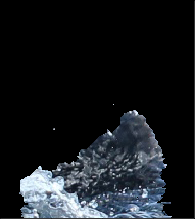
\includegraphics[scale=0.6]{Chapter3/figs/grabcut-example.png}
	\end{center}
	\caption{An example manual crop showing the result of GrabCut background removal.
	}
	\label{fig:grabcut-example}
\end{figure}

As can be seen, the use of GrabCut as a background removal tool does not perform as expected on data the detector is required to operate on. Because of this, as well as the unsuitability of feature extraction as seen in Section \ref{ch:cetDet,sec:deciding,sub:boundingBoxInvestigation,subsub:SIFT}, the use of bounding boxes in the cetacean detector stage was deemed not to be possible. As such, the focus of testing moved to the use of pixel-wise mappings and instance segmentation.  

\subsection{Instance Segmentation Architectures}\label{ch:cetDet,sec:deciding,sub:instanceSegArchitectures}

One of the major decisions that must now be made is which model architecture should be utilised in order to provide the required pixel-level detections. As this project is devoted to improving existing procedures and introducing deep learning to a novel application domain, it is far more advantageous to utilise existing model architectures rather than develop a custom one. The development of a custom architecture for this stage of the project would be extremely time consuming, taking away from more novel parts of the project (notably the identification of the individual animals). Further, as this project is introducing deep learning methods to an application domain where it is not commonplace, the project needs to be able to convince researchers in the space that the system is reliable; this is more easily achieved using a pre-existing architecture where use cases already exist in literature and business. 

To this end there are two main model architectures that can be considered for this task; U-Net \cite{ronneberger_u-net_2015} and Mask-RCNN \cite{he_mask_2017}. Both of these architectures work in different ways. Vuola \textit{et al.} provide a more detailed comparison between the two models \cite{vuola_mask-rcnn_2019}, however the main focus for this project is their resultant output mask structure. 

U-Net is based on an encoder-decoder architecture. This allows for fast and simple segmentation when working with images where only one output is required. For example taking U-Net's original use case of biomedical imaging, the model is able to efficiently segment a group of cells into individual components through boundary estimation to locate the outer edges of the cells. This allows them to be segmented from each other. However this results in an output of the same dimensions as the input, that is, all segmentations are provided in a single binary mask. 

In contrast, Mask-RCNN utilises a multi-stage architecture (described in more detail in Section \ref{ch:Background,sec:instanceSegmentation,sub:Mask R-CNN}) allowing the model to place each detection on its own binary output mask. This is extremely important for the outlined use case. As the detector will be used as part of a larger system for automatic photo-id, any detections made will need to be passed to the identifier as a stand-alone image. If U-Net was utilised for the detection stage, whilst initially being more efficient than Mask-RCNN, further processing of the binary output mask would still be required to split this into it's individual components. In contrast, if Mask-RCNN was utilised then the processing required in between the detection and identification stage would be far simpler. Again, this allows for more time to be spent working on the novel aspects of this project whilst keeping the pipeline as simple as possible. This reason was a big factor in deciding to focus on Mask-RCNN for this stage.

Another factor which must be decided upon when starting development of a deep learning system is the language and framework to be used for development. With regards to language this was a fairly easy decision; a large proportion of deep learning research and development is written in Python. The language benefits from an efficient and lightweight syntax as well as having a host of different deep learning packages available to aid in development. Further to this, both of the major deep learning frameworks, Google's Tensorflow \cite{abadi_tensorflow:_2016} and Facebook's Torch (of which PyTorch is the most actively developed) \cite{paszke_automatic_2017}, both provide full Python support and have active communities for the language. Thanks to this, the vast majority of deep learning development is performed using Python in one of these two frameworks. By utilising these technologies, this project's code is easily reproducible and understood, as well as extendable in the future.

Of the two main frameworks, the use of Tensorflow was decided for the project at this stage. Whilst this decision was made somewhat due to personal preference, Tensorflow was (at least at the time of starting this project) the primary framework for development of deep learning systems outside of academia. Rather than developing a custom Mask-RCNN in Tensorflow for this project, Matterport's Mask R-CNN implementation \cite{waleed_mask_2017} has been adapted.

\section{Initial Testing of Mask-RCNN}\label{ch:cetDet,sec:initialTesting}

In order to build a Mask-RCNN detector which fulfilled the requirements as laid out in Section \ref{ch:cetDet,sec:requirements} an understanding of the framework needed to be achieved. Thankfully, the downloaded repository also includes some tutorial notebooks, most notably an example on balloon segmentation which proved invaluable for learning the basics of how Mask-RCNN operates both on a fundamental code level and at a higher level, understanding how the code can be adapted for other use-cases. In order to progress onto cetacean detection however, a dataset of cetaceans would be needed. 

Exploration of available open-source datasets to find cetaceans in conditions this detector would be operating in proved unfruitful. Many standard benchmarking datasets contain animal classes, and thus an exploration of these was conducted. Of the more generalised benchmark datasets, those such as ImageNet \cite{deng_imagenet:_2009} which contain a large corpus of varied classes, only CIFAR-100 \cite{krizhevsky_learning_2009} contains a \texttt{dolphin} class. However, images in CIFAR-100 are only 32x32 pixels in size, too small to be useful for the task at hand. 

Moving the search away from generalised datasets and towards those which are targetted at conservation efforts or the natural environment also proved fruitless. A large portion of these datasets focus on camera traps or land-based fauna, such as iWildCam \cite{beery_iwildcam_2019}, for reasons discussed in more detail in Section \ref{ch:Background,sec:conTech}. Some images included in the iNaturalist dataset \cite{van_horn_inaturalist_2018} are of cetaceans, such as a class for the short-beaked common dolphin (\textit{Delphinus delphis}), however most focus on other aquatic animals such as the Florida manatee (\textit{Trichechus manatus}), various amphibians, and molluscs. 

\subsection{The Zanzibar Dataset}\label{ch:cetDet,sec:initialTesting,sub:zanzibar}

Due to the lack of open-source and published datasets to aid in the development of this cetacean detector, one was required to be created. As the focus of this project as a whole was the utilisation of the developed system to aid in conservation efforts of resident cetacean populations off the Northumberland coastline, ideally the created dataset would come from this area. At the time of initial testing however this was not possible due to a lack of available data from the survey area.

As such, alternative data was provided by Newcastle University's Marine MEGAfauna Lab. The dataset was curated during a 2015 conservation effort undertaken in Zanzibar, Tanzania, to determine the status of Indo-Pacific bottlenose dolphins in the area \cite{sharpe_indian_2019}. The catalogue provided consisted of 1021 images of size 5184x3456, and was supplied in a format suitable for manual photo-identification rather than for the training of a neural network. Work was then undertaken to convert this conservation catalogue into a machine learning dataset. 

In order to perform this conversion, the provided images must first be labelled. This was achieved using the VGG Image Annotator software, known as VIA \cite{dutta_via_2019}. Other labelling software such as LabelImg \cite{tzutalin_labelimg_2021} were examined, however VIA was deemed the best choice for the task at hand. This software was chosen for multiple reasons; first, the software is noticeably easy to use and allows for efficient labelling on a per-pixel basis as required by Mask-RCNN. Second, the tutorial data provided by the Mask-RCNN Github repository was labelled in VIA format, showing that this code implementation would accept data labelled in this format. Furthermore, use cases of VIA being utilised for labelling of marine-oriented data are available in literature \cite{nita_cnn-based_2020}, providing evidence of suitability of the labelling software for research purposes and data representing similar conditions.

Before labelling the Tanzania data, some curation was performed. Each image labelled by VIA is required to contain at least one non-background class. As such, any images provided which did not contain an example of a \texttt{dolphin} class were discarded. Other images where the class examples were unsuitable for training a Mask-RCNN model, such as those which contained only an extremely small section of the photographed dolphin or were deemed too blurry, were also removed. This left 312 images which were suitable for the Mask-RCNN.

The process for labelling the data with VIA is rather straightforward. The software runs locally through a web browser, with each image labelled sequentially. Figure \ref{fig:via-json-example-zanzibar} shows an example image labelled using VIA. Each image is shown on-screen to the user who is then able to trace around class examples by selecting multiple points on the image. Once a full trace has been performed, any pixels inside of the trace are treated as one class. This class is labelled through the use of a class attribute, in the case of the Tanzania data this was the class label \texttt{fin}, denoting the class example as a fin above the waterline. These labels are stored in a corresponding JSON file, which is fed to the Mask-CNN model along with the images during training. This labelling allows the model to learn per-pixel class examples during training. This tracing method also allows for each distinct individual in a group to be labelled individually, even if overlapping, which would be much harder to perform with bounding box labelling and allows the model to learn how to differentiate between group members.  

  \begin{figure}
	\begin{center}
		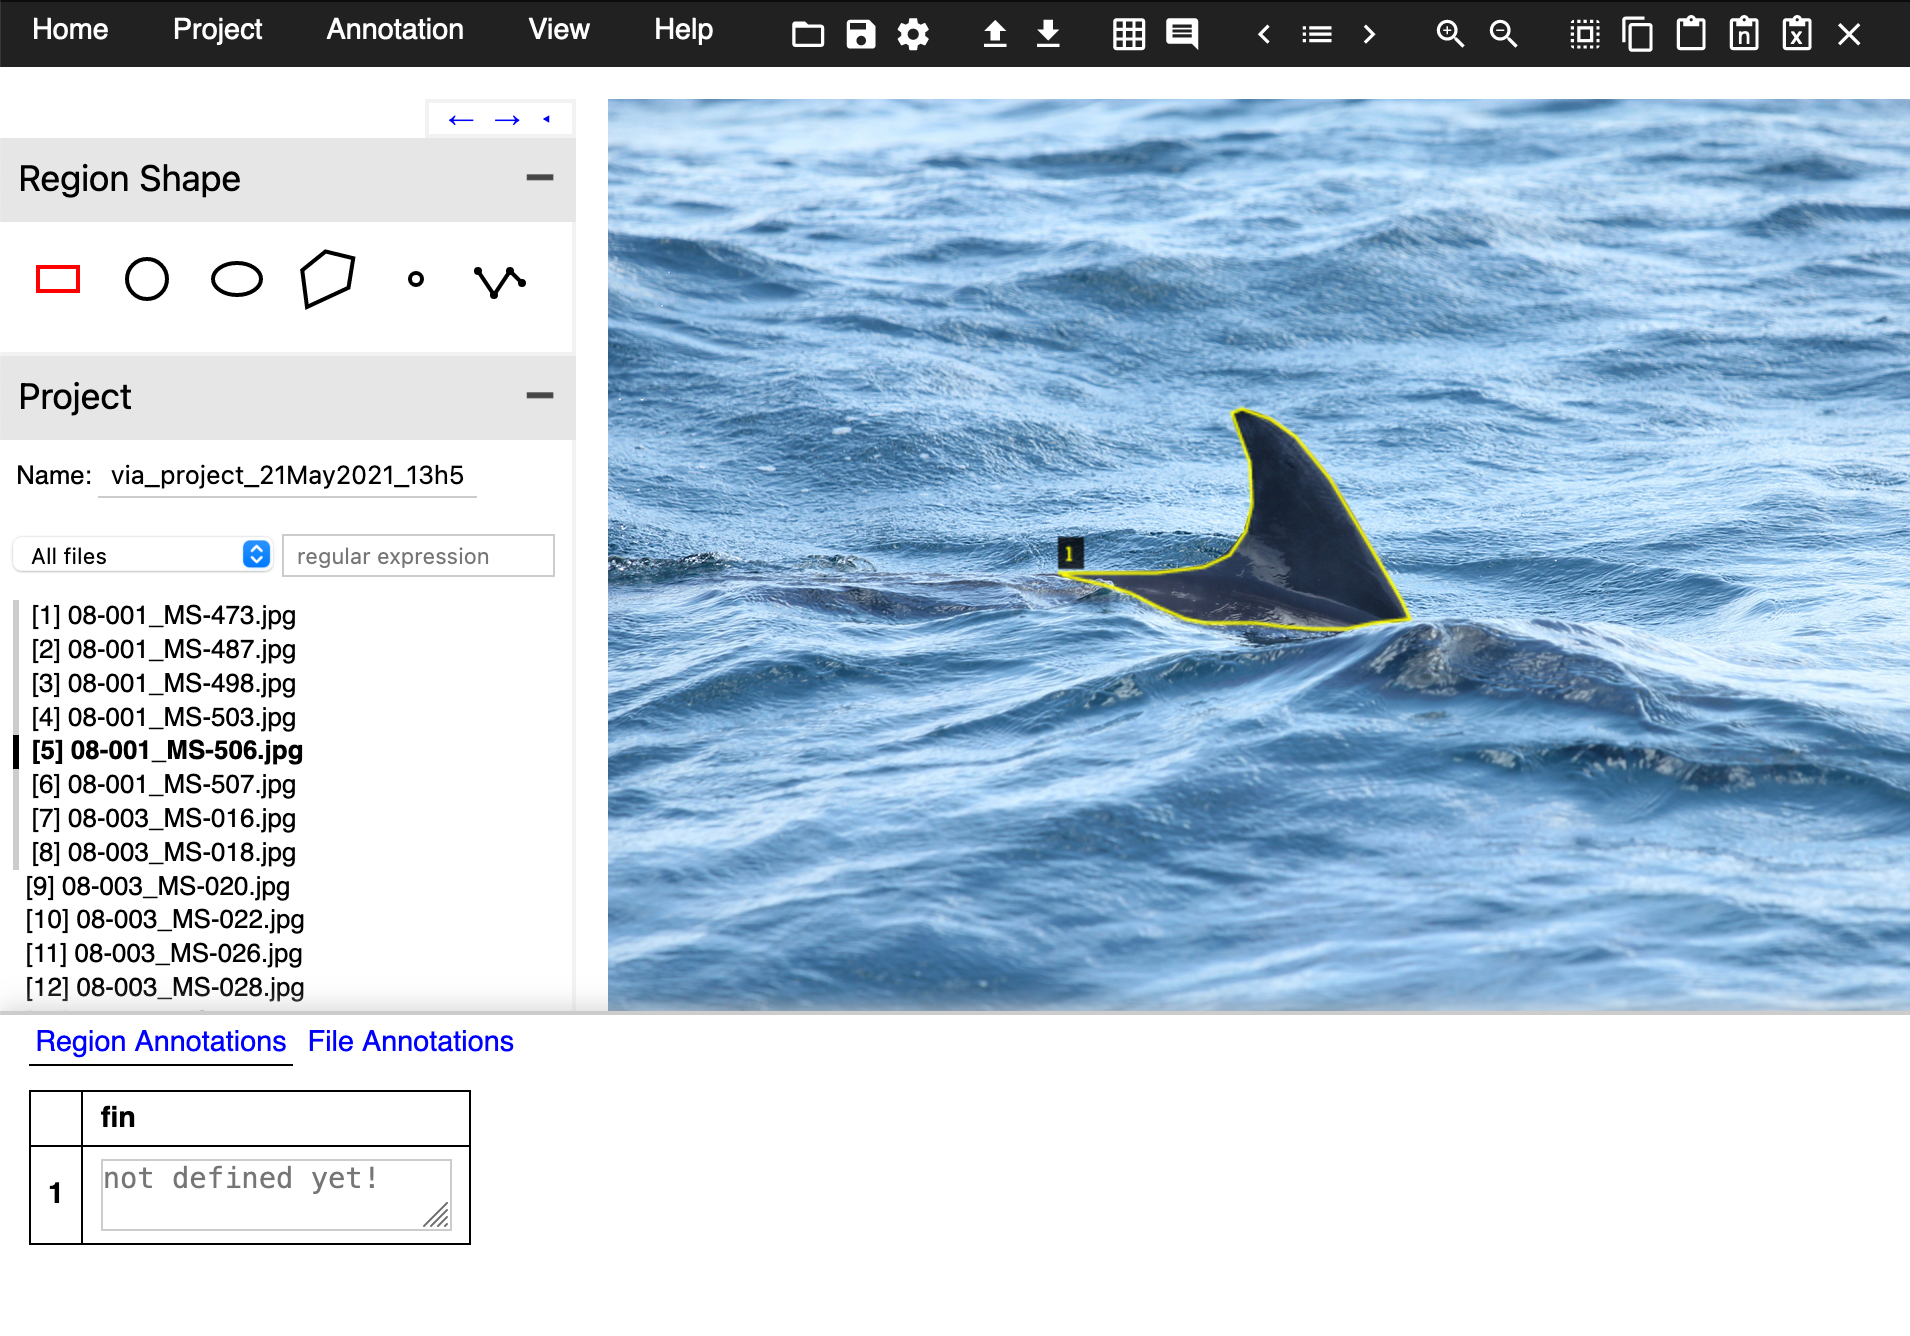
\includegraphics[scale=0.4]{Chapter3/figs/via-json-example-zanzibar-1.png}
	\end{center}
	\caption{An example image showing the labelling processes using VIA.
	}
	\label{fig:via-json-example-zanzibar}
\end{figure}

Once all 312 images had been labelled, it was then possible to create a train-test split. The 312 images were divided using an 80-20 split, where 80\% of the images are designated for training the Mask-RCNN model, known as the training set, and the remaining 20\% were held back for model evaluation, known as the test set. By evaluating on previously unseen data this affords researchers the ability to understand the generalisability of the trained model, mitigating overfitting. 

This newly created Zanzibar dataset would allow for prototyping to begin, determining the suitability of a Mask-RCNN based model for the task of a cetacean detector. The Zanzibar dataset was very similar in content to what would be expected from a dataset created from North Sea survey data once this had taken place and thus gave a good baseline for experimentation. 

\subsection{Transfer Learning}\label{ch:cetDet,sec:initialTesting,sub:transferLearning}

Whilst the Zanzibar dataset provides experimental data similar to that which the Mask-RCNN model will be required to process, the amount of data is extremely small. Deep learning models often require thousands of images when training to produce generalisable and accurate models. As such, this dataset alone would not be enough to train the cetacean detector. One way to approach this issue would be to locate more photo-id data. However, little extra data was readily available from the Marine MEGAfauna Lab, and data from other labs would require a large amount of effort to obtain. Cetacean catalogues are closely guarded by conversation labs due to the large amount of effort required to obtain them. Second, any further data collected would also need to be labelled and incorporated into the now existing dataset, which again would require significant time and effort. These issues rendered the prospect of expanding the Zanzibar dataset unachievable in the time required. 

Another approach available is the concept of transfer learning. This is a technique whereby models trained to perform one task are repurposed to aid in a second, usually more specialised task. These initial models have typically been trained on large generalised datasets such as ImageNet \cite{deng_imagenet:_2009} or Microsoft's Common Objects in Context, more commonly known as MSCOCO \cite{lin_microsoft_2014}. These datasets often contain hundreds of thousands of images covering a large number of classes, which make them perfect for the task of transfer learning. 

By first training a model on these large datasets, the model is able to learn the basics of image understanding, for example the concept of basic shapes and colour, allowing for the development of a generic visual understanding model. By utilising these models, we effectively provide our own model with a head-start in its learning process, there is no need to utilise the small amount of data available in the Zanzibar dataset for low level learning; it can instead be saved for allowing the model to understand and generalise to the domain specific task, such as cetacean detection. For a more in-depth analysis of transfer learning, see Pan \textit{et al.} \cite{pan_survey_2010}.

Training a neural network, or model, is extremely computationally and time expensive due to the large dataset sizes used. As such, many models suitable for transfer learning can be obtained in a pre-trained state. These pre-trained models are hosted by model zoos, which provide frozen model weight files in a format which allow for transfer learning to take place through a process known as fine-tuning. Here, a model from the zoo is downloaded and \textit{n}-number of deeper layers are unfrozen. Next, additional layers are added to the model which perform the domain specific task. The unfrozen and additional layers are then trained on the domain specific task, allowing for the fine-tuning of the higher-level feature extraction. 

\subsection{Utilising Transfer Learning to Train the Mask-RCNN}\label{ch:cetDet,sec:initialTesting,sub:transferLearningforTheDetector}

The use of transfer learning can be easily adapted for the training of the cetacean detector for use with the Zanzibar dataset, achieved directly through Tensorflow. First, a backbone model architecture is chosen. For the cetacean detector, it was decided that a ResNet50 backbone would be utilised. Matterport's Mask-RCNN implementation allows for the use of a ResNet50 or ResNet101 backbone, both standard variants of ResNet which are 50 and 101 layers deep respectively \cite{he_deep_2015}. ResNet50 was chosen over ResNet101 as during initial experimentation with the Matterport provided tutorial data, no significant improvement in accuracy was achieved using the deeper 101 layer model although a significant increase in training time was observed.

Once a backbone architecture was chosen, it can then be loaded into Tensorflow. Next, the pre-trained model weights are downloaded from the model zoo. These weights denote the strength of the connections between the model's layers. In the case of a model being trained from scratch without transfer learning, the weights of each layer are randomly initialised and then manipulated through backpropagation to achieve a desired model output. 

In transfer learning however, the model's starting weights are not initialised randomly. Instead, the weights of the trained network hosted on the model zoo are used as a starting point. This replicates the final state of the model trained on the larger dataset. 

As previously mentioned, there are multiple different models available in the zoo, all trained on a large variety of benchmark datasets. Each dataset produces a model with different final trained weights. Before applying transfer learning to the ResNet50 architecture chosen it is important to make an informed decision as to which benchmark dataset the model should be initialised from. 

For this project it was decided that the ResNet50 weights trained on MSCOCO \cite{lin_microsoft_2014} would be utilised. This was due to the fact that MSCOCO is primarily an instance segmentation dataset, and thus one of the most appropriate to use for transfer learning to another instance segmentation task. The use of MSCOCO for pre-training on Mask-RCNN has in recent years been well documented in literature for a variety of tasks \cite{yu_fruit_2019, couteaux_automatic_2019, fujita_fine-tuned_2020} including in land-based photo-id system, with Kulits \textit{et al}. utilising MSCOCO as a transfer learning dataset when training a modified Faster-RCNN system for African elephant re-identification \cite{kulits_elephantbook_2021}. As Mask-RCNN builds on Faster-RCNN, it was deemed reasonable to assume MSCOCO would also work well for pretraining a Mask-RCNN based system.

When utilising an MSCOCO pre-trained architecture for a Mask-RCNN based task, it is important to note that certain layers must be excluded when loading in the pre-trained weights as these are only utilised in Mask-RCNN models, such as those which deal with the per-pixel masks. This is because these layers require the same number of neurons as dataset classes, similar to a fully connected layer. If the MSCOCO weights were utilised at these final layers for the task at hand there would be a mismatch between the number of classes in MSCOCO, 80, and in the Zanzibar dataset, 1 (plus \texttt{background}).

Once the backbone architecture has been loaded with pre-trained weights, the total number of layers to fine-tune must be decided. This can be considered similar to a hyperparameter, as it must be chosen at run time by the user. Whilst any number of the layers can be chosen for fine-tuning, only the model heads are selected. These are layers required for the Region Proposal Network, the pixel classification, and masking layers of the model. For the purposes of hyperparameter tuning, whether the model weights are randomly initialised or loaded from a pre-trained model can be selected.

\subsection{Data Augmentation}\label{ch:cetDet,sec:initialTesting,sub:dataaugmentation}

As well as transfer learning the use of data augmentation was also explored to help mitigate the issue of dataset size. This technique allows for datasets to be artificially expanded by performing random perturbations to each data point which are then automatically class labelled the same as the original input. Figure \ref{fig:data-aug-examples} shows examples of data augmentations found in literature.

\begin{figure}[h]
	\begin{center}
		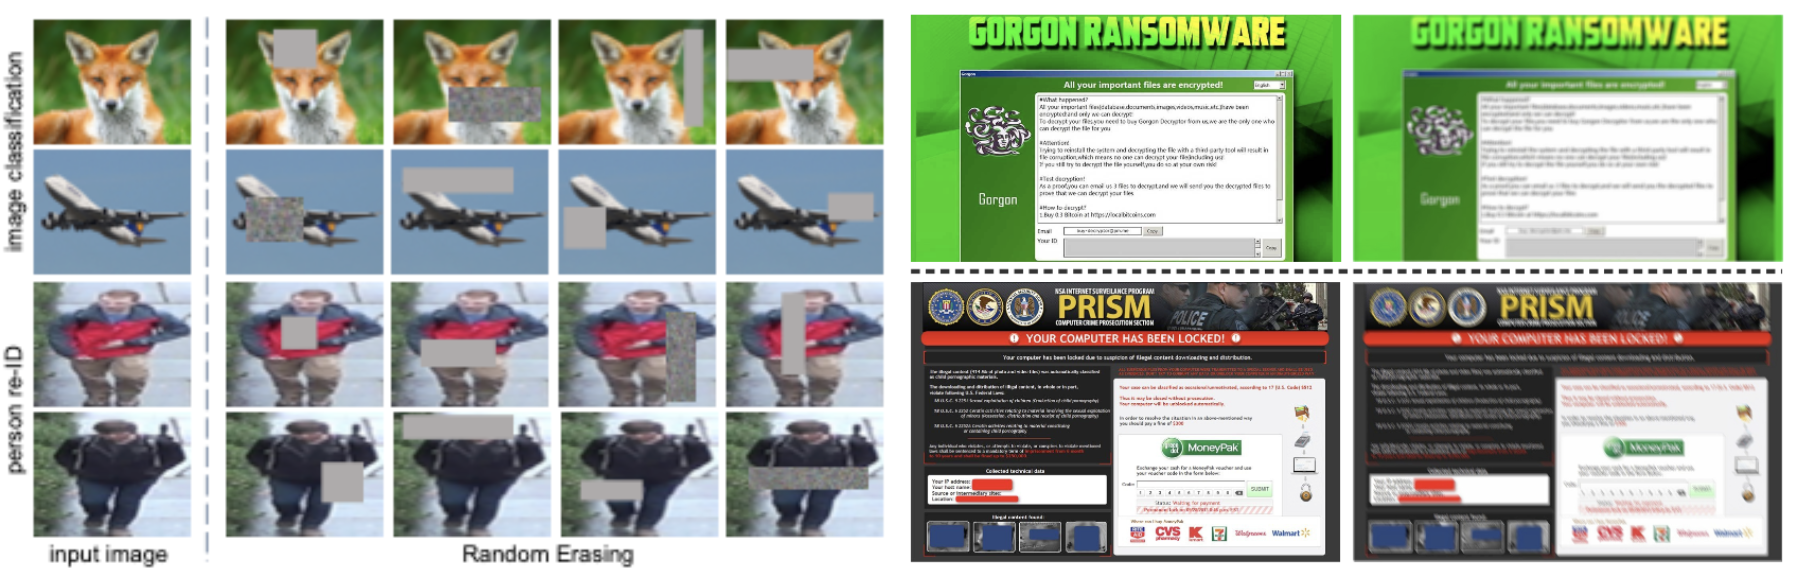
\includegraphics[scale=0.45]{Chapter3/figs/data-augs.png}
	\end{center}
	\caption{Examples of data augmentations found in literature. Left: Randomly erasing parts of images, from Zhong \textit{et al}. \cite{zhong_random_2017}. Right: Augmentations to simulate screenshot capture. Defocus blur (top), motion blur (bottom) from Atapour-Abarghouei \textit{et al}. \cite{atapour-abarghouei_kings_2019}.}
	\label{fig:data-aug-examples}
\end{figure}

When augmenting data it is extremely important to understand a dataset's problem domain to ensure that any transformations are realistic and expose the model trained to data which, whilst not present in the dataset before augmentation, could still reasonably expected to be seen by the model when deployed. Further, augmentation must only occur on the training data and not the test data. This is in contrast to preprocessing techniques such as resizing, which must occur to all data points. 

As the Zanzibar data contains relatively few images, it is a prime candidate for data augmentation. This can be performed in one of two ways; in either an offline or an online manner. In offline data augmentation, the entire train split is augmented before the images are passed to the model, occurring as a preprocessing step. This is extremely useful for very small datasets where the number of examples needs to be increased before the model can begin training, or if training time is a concern. The major issue with offline augmentations however is that, because the data is perturbed and then passed to the model, offline augmentation produces a fixed number of augmented images. 

This can be solved with online augmentation, which occurs in real-time as the model trains. The model is passed the original, unperturbed data which is then augmented during each training batch. This allows for the model to see a potentially unlimited number of `new' images, as each input image is randomly perturbed before being used for training. Once training on the batch has been completed, the augmented images are discarded and new perturbations performed. As such online augmentation is, if possible, greatly preferred and allows for a much higher chance of model generalisation. 

Whilst the Zanzibar dataset is small compared to many others used for deep learning, it is large enough to allow for online augmentation. In order to begin testing the effect of data augmentation on the Mask-RCNN training process, two different augmentation strategies were created which contained unique workflows. 

The first strategy, \textit{aug1}, selected between zero and three of the following perturbations: (1) \textit{horizontal flip}: flip the image horizontally with a probability of 0.5, (2) \textit{vertical flip}: flip the image vertically with a probability of 0.5, (3) \textit{rotation}: rotate the image either 90, 180, or 270 degrees each with equal probability of occurring, (4) \textit{scaling}: scale the image between 80\% and 120\% on both axis independent of each other, (5) \textit{brightness}: multiply all pixels in the image with a random value between 0.8 and 1.5, (6) \textit{Gaussian blur}: blur the image with a Gaussian kernel with radius randomly assigned between 0 and  5. 

The second strategy, \textit{aug2}, was more complex, performing the following perturbations in a sequentially random order on 67\% of the images only: (1) \textit{horizontal flip}: flip the image horizontally with a probability of 0.5, (2) \textit{cropping}: crop each side of the image randomly between 0\% and 10\% of the total side length, (3) \textit{Gaussian blur}: blur the image with a Gaussian kernel with radius randomly assigned between 0 and 2.5, with a probability of blurring of 0.5, (4) \textit{contrast}: strengthen or weaken the contrast of the image by a random factor between 0.75 and 1.5, (5) \textit{additive Gaussian noise}: sample the noise per channel - adding noise to the colour of the pixels, (6) \textit{brightness}: multiply all pixels in the image with a random value between 0.8 and 1.2, (7) \textit{scaling}: scale the image between 80\% and 120\% on both axis independent of each other, (8) \textit{rotation}: rotate the image randomly between -180 and 180 degrees. 

The use of two augmenters allowed for evaluation on whether a simple or more complex augmentation strategy would be appropriate for this use case. By using multiple augmenters we can treat them as a hyperparameter of model training, allowing the augmenter chosen to be added to the search space.

\section{Mask-RCNN Model Selection}\label{ch:cetDet,sec:ModelSelection}

When training a Mask-RCNN model there are a large range of hyperparameters, or user defined values, which must be set before training can occur. These hyperparameters each have influence on the final model's performance, and can be broken down into two subgroups; detection hyperparameters influence the output of the model, and training hyperparameters which influence the training of the model. Thankfully most deep learning frameworks provide default values for most, if not all hyperparameters. These default values are known to work well regardless of dataset or task, and so many have been used when training the Mask-RCNN. Some hyperparameters however can have a large effect on the final model and so an exploration of the optimal value for these has been undertaken with the goal of producing the optimal overall model for the task of cetacean detection, both on the Zanzibar dataset and on other similar datasets. 

\subsection{Detection Hyperparameters}\label{ch:cetDet,sec:ModelSelection,sub:DetectionHyperparameters}
 
 With regards to the detection hyperparameters, only the minimum confidence of the model was changed from the default of 0.7 to 0.9. This was changed as during initial trials it was found models trained on the Zanzibar data would often produce a high number of false positives (for example detecting a wave as a fin) or create duplicate detections (one fin detected twice). By increasing the minimum confidence of the model to 0.9, we increase the threshold at which the model returns a detection to 90\%, or in other words for every detection the model must be 90\% sure that the detection is actually a fin before notifying the user. This reduced both the false positive rate and duplicate detection rate of the model. An example of this can be seen in Figure \ref{fig:min-conf}. Note how in the left image more detections are present than in the right image, however the extra detections are either part of an existing detection (yellow) or do not contain enough fin to identify the individual (red).
 
\begin{figure}[h]
	\begin{center}
		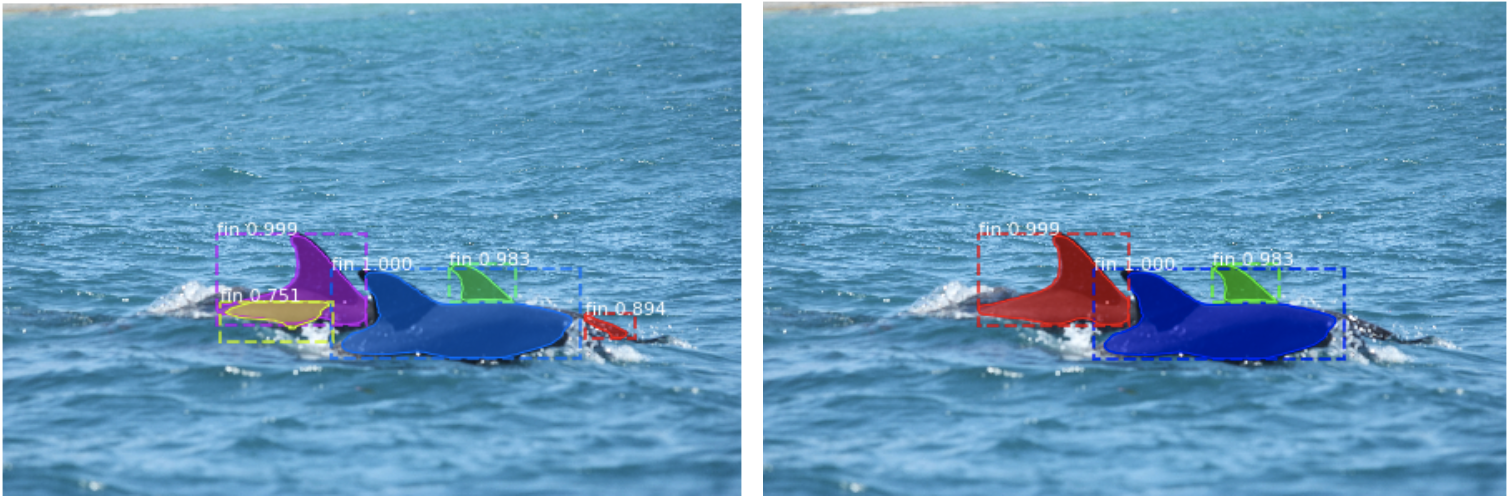
\includegraphics[scale=0.55]{Chapter3/figs/min-conf-eg.png}
	\end{center}
	\caption{An example image showing the effect of minimum detection confidence thresholding in Mask-RCNN detections. Left: A threshold of 0.7. Right: A threshold of 0.9.}
	\label{fig:min-conf}
\end{figure}
 
 
\subsection{Training Hyperparameters}\label{ch:cetDet,sec:ModelSelection,sub:TrainingHyperparameters}

The vast majority of hyperparameters influence the training process. Selection of the optimal hyperparameters is however an extremely computationally and time expensive task, as the optimal values of the hyperparameters are not known before training begins. Indeed, even after training has finished and a model which produces satisfactory results has been found there is no guarantee that the hyperparameters of this model are the best, just that they were the best found so far. 

As such, in order to determine the best hyperparameters for a given model and task, the search space of all possible hyperparameters must be searched. This is infeasible due to time and resource constraints however,  therefore a technique known as grid searching was performed. During a grid search, each of the possible hyperparameters will have a range of values defined. A model is then trained using the data and each combination of defined hyperparameter values. Once each model has been trained, they are then evaluated to determine the best hyperparameters. In some cases an acceptable model will be found during the initial grid search, however this may not be the case. In this situation the previous grid search may not be useless, as it may provide insight into how to refine the search space to increase the chances of an acceptable model being trained. This process of finding the optimal hyperparameters for the model is known as hyperparameter tuning. 

\subsubsection{Learning Rate Scheduling \& Optimisers}\label{ch:cetDet,sec:ModelSelection,sub:TrainingHyperparameters,subsub:learningRateOptimisers}
One of the most important hyperparameters to tune is the learning rate, which dictates how much the weights of the model should change in response to the estimated error calculated during backpropagation. If the learning rate is too large this will lead to an unstable training process whereby gradient descent can never reach the minimum value but rather bounce either side of it. If the learning rate is set too small the training process will take an extremely long time to converge. 

In order to help the model reach its optimal minima in a reasonable time, the learning rate can be adjusted using a scheduler. These allow for the learning rate to be modified when some criteria is met, such as after a set number of epochs, allowing for larger weight changes initially for fast training before reducing the descent steps as time goes on, decreasing the chance of gradient descent jumping over the minima.

As well as learning rate schedulers, adaptive rate optimisers can also be used. These optimisers provide an alternative to SGD (an overview of which can be found in Section \ref{ch:Background,sec:DLIntro,sub:stochasticgradientdescent}) and are capable of adapting to the dataset it is given and the current training process, changing the learning rate without a defined schedule. This often allows for a more optimised and efficient training process when compared to using SGD, as discussed in Section \ref{ch:Background,sec:DLIntro,sub:stochasticgradientdescent}. During hyperparameter tuning of the Mask-RCNN, two optimisers were chosen for evaluation. 

The first, SGD with restarts (SGDR) \cite{loshchilov_sgdr:_2016} allows for decreases in the learning rate through a process known as cosine annealing, whereby the decrease follows a cosine waveform. This results in a high starting learning rate allowing for a fast approach to a local minima before reducing the rate as the number of epochs increases to prevent a jump over the minima, similarly to how a scheduler works. However it may not be the case that this local minima is the global minima, the lowest possible point in the space. Due to cosine annealing it would not be possible to leave the local minima, the learning rate needs to be increased again to allow for this. As such the learning rate is \textit{restarted}, or increased back to its maximum, to allow for the training process to jump out of the local minima; if it is indeed the case that this local minima is also the global minima then the training process will return to the point it was at before the restart, however if the local minima was not the global minima, the restart will allow for the training process to leave the sub-optimal minima it previously found. 

The second learning rate optimisation explored during hyperparameter tuning is Adam, or adaptive moment estimation. This optimiser is extremely popular in the world of deep learning \cite{karpathy_peek_2017}, capable of achieving impressive results in relatively short training times. This is possible through the use of one learning rate for each model weight, in contrast to the singular learning rate for the whole model as seen in SGD or SGDR. Adam also utilises parts of other optimisers such as AdaGrad \cite{duchi_adaptive_2011} and RMSProp \cite{tieleman_lecture_2012} to allow the optimiser to work well with both sparse and noisy data. For a complete breakdown of the inner workings of Adam, see Kingma \textit{et al}. \cite{kingma_adam:_2014}. 

\subsubsection{Weight Decay}\label{ch:cetDet,sec:ModelSelection,sub:TrainingHyperparameters,subsub:WeightDecay}

The goal of neural network development is to utilise the training data in such a way that the resulting generated model performs well on unseen data. In order for this to be achieved our model must be generalisable, having learnt enough from the training data to perform well at the given task but not having learnt so well that it is unable to perform adequately on unseen data. If a model fails to generalise, it is said to have overfitted the data. For example lets say we wish to develop a cat detector, a model which given an input image will tell you if there is a cat present. However, we only train our model on images with white cats in them. The model trains well, and is always able to tell you if there is a cat in the images it sees during training. When deployed, the model fails to identify any images containing black cats - the model has learnt the training data too well and believes cats can only be white; the model has overfitted. 

There are many different techniques to reduce overfitting in neural networks, one of the easiest is to simply collect more training data. As previously mentioned, due to how closely guarded cetacean photo-id catalogue data is and how expensive it is to collect, this was not possible. As such, the use of weight decay was explored during hyperparameter tuning. Weight decay is a regularisation technique which allows the model training to be penalised in proportion to the size of its weights. This incentivises the training process to keep the weights small, which has been shown to improve generalisation to unseen data \cite{krogh_simple_1991}. As the Zanzibar dataset is comparability small compared to the usual size of datasets for this task, allowing the model to generalise well using small amounts of data is extremely important.

\subsubsection{RPN Anchor Scales}\label{ch:cetDet,sec:ModelSelection,sub:TrainingHyperparameters,subsub:RPNAnchorScales}

As discussed in Section \ref{ch:Background,sec:objectDetection,sub:RPN}, Region Proposal Networks (RPNs) can be utilised in object detection due to their ability to determine potential regions of interest (RoIs) in the image, known as anchors. These anchors are then classified as either \texttt{background} or of a learnable class, such as \texttt{dolphin}. To allow the RPN to be object-size invariant, anchor scales are utilised. These scales, provided as a list of values which correspond to the square anchor side in pixels, determine what sizes the RoIs proposed by the RPN should be. For example, let's say an anchor scale of \texttt{[32]} is passed to the RPN, this would mean that all RoIs proposed by the RPN would be of size 32x32 pixels. The anchor scale provided to the RPN can be considered a hyperparameter as the best scales for the RPN to allow for the detection of objects regardless of their size must be determined. 

\subsection{Hyperparameter Tuning via a Grid Search}\label{ch:cetDet,sec:ModelSelection,sub:HyperparameterTuning}

Although only a few hyperparameters have been chosen to tune, the size of the possible search space to evaluate is still extremely large. As mentioned previously, it is not feasible both from a time and resource perspective to evaluate the entire space and find the truly optimal value for each hyperparameter. Instead the search space is discretised using a grid search, for each hyperparameter a subset of possible values is selected. Each combination of hyperparameter values is then evaluated to determine which set of values produces a satisfactory model. 

The list of possible hyperparameter combinations and model name, determined by the datetime value at the start of the model's training run, can be seen in Table \ref{tab:MaskRCNNHyperparamTuningGridSearch}. This reduced hyperparameter tuning run still required significant amount of time and resources, running over three NC12 Microsoft Azure VMs, each with two Tesla K80 GPUs, taking approximately one week to complete the grid search producing a total of 50 models. Model runs were split between the VMs based on augmentation strategy with one VM running only \textit{aug1}, the other \textit{aug2}, and the final with no augmentation strategy. It should be noted here that this computational and time expense would most likely be reduced should the images used to train the Mask-RCNN not be so large, although the reasons for this decision are discussed in Section \ref{ch:cetDet,sec:requirements,sub:technical}.

\begin{table}[!ht]
	\tiny
	\begin{adjustbox}{width=\columnwidth, center}
		\begin{tabular}{cccccc}
			\toprule
			Model Name & Weight Decay &        RPN Anchor Scales & Optimiser & Augmentation Strategy & Pre-trained on MSCOCO? \\
			\midrule
			20190829T1458 &         0.01 &   (16, 32, 64, 128, 256) &      Adam &                  aug1 &                  True \\
			20190829T2020 &         0.01 &   (16, 32, 64, 128, 256) &      Adam &                  aug2 &                  True \\
			20190830T0145 &         0.01 &   (16, 32, 64, 128, 256) &      Adam &                  None &                  True \\
			20190830T0714 &         0.01 &   (16, 32, 64, 128, 256) &      Adam &                  aug1 &                   False \\
			20190830T1443 &         0.01 &   (16, 32, 64, 128, 256) &      Adam &                  aug2 &                   False \\
			20190830T2019 &         0.01 &   (16, 32, 64, 128, 256) &      Adam &                  None &                   False \\
			20190902T0946 &         0.01 &   (16, 32, 64, 128, 256) &      SGDR &                  aug1 &                  True \\
			20190904T2004 &         0.01 &   (16, 32, 64, 128, 256) &      SGDR &                  None &                  True \\
			20190905T1813 &        0.001 &  (32, 64, 128, 256, 512) &      SGDR &                  aug1 &                  True \\
			20190905T1826 &         0.01 &   (16, 32, 64, 128, 256) &      SGDR &                  aug2 &                  True \\
			20190905T2202 &        0.001 &  (32, 64, 128, 256, 512) &      Adam &                  None &                  True \\
			20190905T2336 &        0.001 &  (32, 64, 128, 256, 512) &      Adam &                  aug1 &                  True \\
			20190906T0332 &        0.001 &  (32, 64, 128, 256, 512) &      SGDR &                  None &                  True \\
			20190906T0851 &         0.01 &  (32, 64, 128, 256, 512) &      Adam &                  None &                  True \\
			20190907T0932 &        0.001 &   (16, 32, 64, 128, 256) &      Adam &                  aug1 &                  True \\
			20190907T0933 &       0.0001 &  (32, 64, 128, 256, 512) &      Adam &                  aug2 &                   False \\
			20190907T0934 &         0.01 &  (32, 64, 128, 256, 512) &      SGDR &                  None &                  False \\
			20190907T1451 &        0.001 &   (16, 32, 64, 128, 256) &      Adam &                  None &                  True \\
			20190907T1500 &       0.0001 &  (32, 64, 128, 256, 512) &      Adam &                  aug1 &                   False \\
			20190907T1545 &         0.01 &  (32, 64, 128, 256, 512) &      Adam &                  aug2 &                   False \\
			20190907T2026 &       0.0001 &  (32, 64, 128, 256, 512) &      SGDR &                  None &                  True \\
			20190907T2126 &        0.001 &   (16, 32, 64, 128, 256) &      Adam &                  aug1 &                   False \\
			20190907T2215 &        0.001 &   (16, 32, 64, 128, 256) &      SGDR &                  aug2 &                  True \\
			20190908T0202 &       0.0001 &   (16, 32, 64, 128, 256) &      Adam &                  None &                  True \\
			20190908T0352 &         0.01 &  (32, 64, 128, 256, 512) &      Adam &                  aug2 &                  True \\
			20190908T0417 &       0.0001 &  (32, 64, 128, 256, 512) &      Adam &                  aug1 &                  True \\
			20190908T0957 &       0.0001 &  (32, 64, 128, 256, 512) &      Adam &                  None &                   False \\
			20190908T1102 &       0.0001 &  (32, 64, 128, 256, 512) &      Adam &                  aug2 &                  False \\
			20190908T1204 &        0.001 &   (16, 32, 64, 128, 256) &      SGDR &                  aug1 &                  True \\
			20190908T1939 &        0.001 &   (16, 32, 64, 128, 256) &      Adam &                  aug2 &                   False \\
			20190908T2043 &       0.0001 &  (32, 64, 128, 256, 512) &      SGDR &                  aug1 &                  True \\
			20190908T2139 &       0.0001 &   (16, 32, 64, 128, 256) &      Adam &                  None &                   False \\
			20190909T0723 &       0.0001 &   (16, 32, 64, 128, 256) &      Adam &                  aug1 &                   False \\
			20190911T1922 &         0.01 &   (16, 32, 64, 128, 256) &      Adam &                  aug2 &                   False \\
			20190912T0045 &       0.0001 &   (16, 32, 64, 128, 256) &      Adam &                  aug2 &                   False \\
			20190912T0608 &       0.0001 &   (16, 32, 64, 128, 256) &      SGDR &                  aug1 &                  True \\
			20191101T1633 &       0.0001 &  (32, 64, 128, 256, 512) &      SGDR &                  aug2 &                  True \\
			20191101T2104 &        0.001 &     (8, 16, 32, 64, 128) &      SGDR &                  aug2 &                  True \\
			20191102T0140 &         0.01 &  (32, 64, 128, 256, 512) &      SGDR &                  aug1 &                  True \\
			20191102T0615 &         0.01 &     (8, 16, 32, 64, 128) &      SGDR &                  aug2 &                  True \\
			20191102T1051 &       0.0001 &   (16, 32, 64, 128, 256) &      SGDR &                  None &                  False \\
			20191102T1528 &        0.001 &  (32, 64, 128, 256, 512) &      SGDR &                  aug2 &                  True \\
			20191102T2006 &       0.0001 &     (8, 16, 32, 64, 128) &      SGDR &                  aug2 &                  True \\
			20191103T0044 &       0.0001 &     (8, 16, 32, 64, 128) &      SGDR &                  aug1 &                  True \\
			20191103T0520 &        0.001 &     (8, 16, 32, 64, 128) &      SGDR &                  None &                  True \\
			20191103T0959 &         0.01 &  (32, 64, 128, 256, 512) &      SGDR &                  aug2 &                  True \\
			20191103T1441 &       0.0001 &     (8, 16, 32, 64, 128) &      SGDR &                  None &                  True \\
			20191103T1921 &       0.0001 &   (16, 32, 64, 128, 256) &      SGDR &                  aug2 &                  True \\
			20191104T0011 &        0.001 &     (8, 16, 32, 64, 128) &      SGDR &                  aug1 &                  True \\
			20191104T0450 &         0.01 &     (8, 16, 32, 64, 128) &      SGDR &                  aug1 &                  True \\
			\bottomrule
		\end{tabular}
	\end{adjustbox}
	\caption{Hyperparameter values used for each grid search run when training the Mask-RCNN model on the Zanzibar data.}\label{tab:MaskRCNNHyperparamTuningGridSearch}
\end{table}

\subsection{Model Selection Based on Grid Search}\label{ch:cetDet,sec:ModelSelection,sub:ModelSelectionBasedOnGridSearch}

Once a grid search has been performed, the results can then be evaluated to determine if a suitable model had been found using the test set. All models trained were evaluated using MSCOCO's Mean Average Precision metric\footnote{COCO mAP Definition: \href{https://cocodataset.org/\#detection-eval}{cocodataset.org/\#detection-eval}}, a commonly used metric for segmentation tasks. This metric, commonly written as mAP@IOU[0.5:0.95], calculates precision-recall graphs for each dataset class at incremental IOU levels, from 0.5 to 0.95 in 0.05 steps. Once each class' precision-recall graph for a given IOU threshold has been calculated, the mean of these values is derived giving an overall mean average precision score for all classes at a given IOU threshold; these thresholds are explained in more detail in Section \ref{ch:Background,sec:semanticSegmentation}.

By evaluating over multiple thresholds the models can then be compared and their performance more easily understood and ranked, as well as allow for the determination of an acceptable loss in IOU overlap. For example if all models were evaluated using mAP@IOU[0.5] only, it may be the case that all models achieve a similar high score, making it difficult to determine which model will be best for the task. However if too high a threshold is used, for example mAPIOU[0.95], it is unlikely that any model will achieve a high score as this would require constant near pixel perfect detection. 

Figure \ref{fig:mAP-graph} shows a visualisation of the mAP@IOU[0.5:0.95] scores for all models trained in the grid search, the raw scores can be seen in Appendix \ref{app:mAPScoresGridSearch}. At mAP@IOU[0.5] there is a large gap in model performance with model 20190830T1443 having the lowest mAP@IOU[0.5] of 0.73 and model 20190905T1813 having the highest at 0.94. This shows that the combination of hyperparameter values provided to the model before training have a significant effect on the model's overall performance, although even the lowest score here is still high. 

At mAP@IOU[0.75], whereby detections would overlap with 75\% of pixels in the ground truth mask, the minimum model performance has dropped significantly with model 20190830T071 achieving a score of 0.49. The highest score at this threshold is model 20191102T0140 with a score of 0.81; this model achieved an map@IOU[0.5] score of 0.92, only two percentage points behind the best model at that threshold. This again shows the need for hyperparameter tuning when selecting models, as they are shown here to have a significant effect on how well the models perform at higher thresholds.

This effect is even greater when comparing map@IOU[0.85] scores, with the worst performing model, 20190830T0714,  achieving a score of just 0.17 whilst the best model, 20190902T0946, achieves a score of 0.50, a difference of 33\%. Model performance drops significantly at the highest threshold with four models achieving an mAP@IOU[0.95] score of 0.016, with most models achieving a score of 0.0. This is to be expected however as it would be highly unlikely that any model, regardless of hyperparameters, would be able to perform near perfect pixel level detections on the test set data. 

\begin{figure}[h]
	\begin{center}
		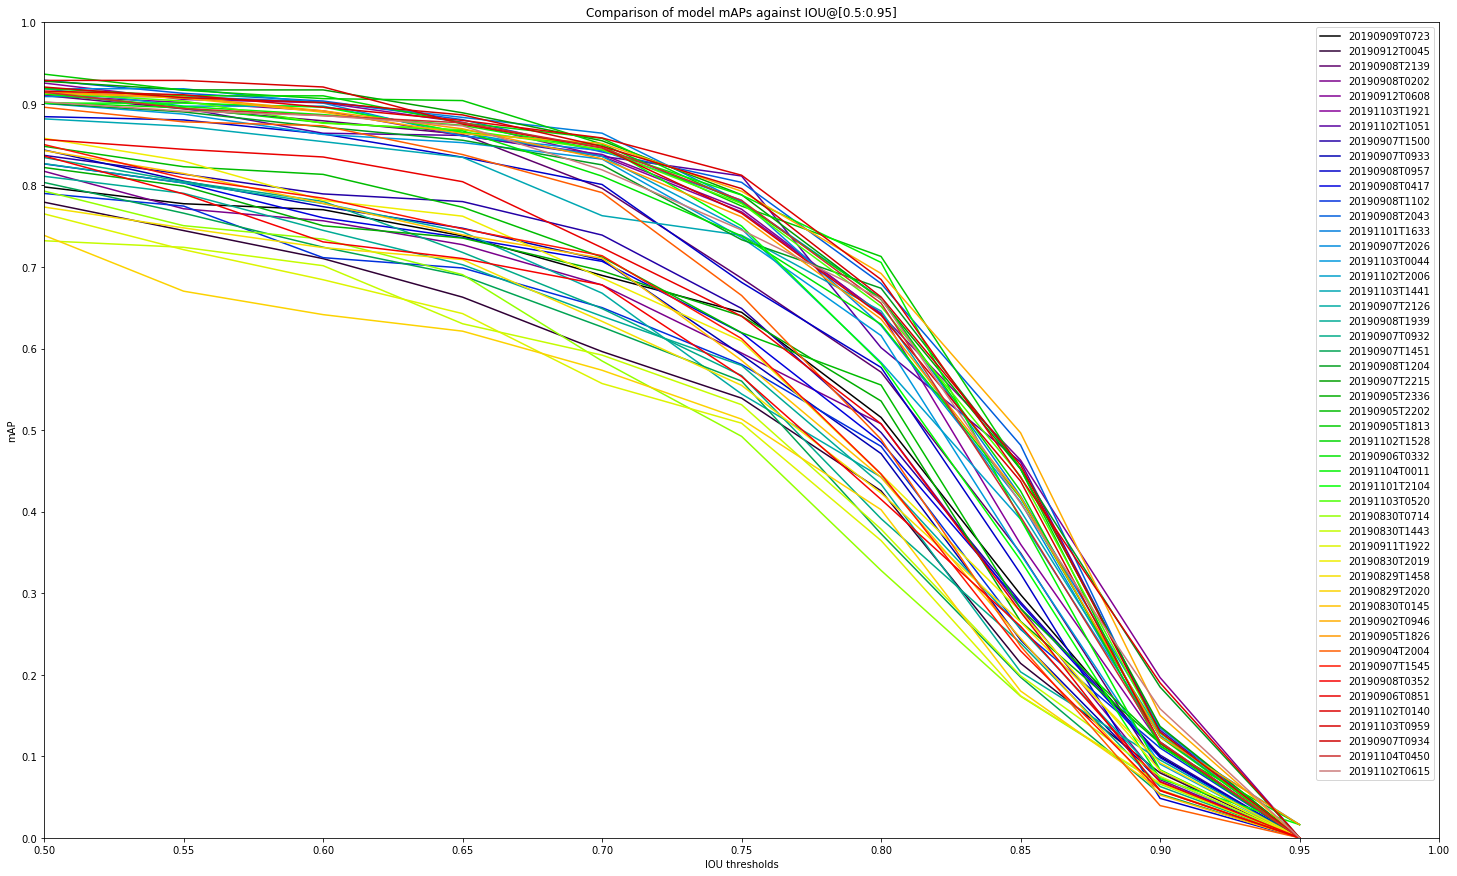
\includegraphics[scale=0.3]{Chapter3/figs/comparison_graph_all_diff_colours.png}
	\end{center}
	\caption{mAP@IOU[0.5:0.95] scores for all models trained in the Mask-RCNN Zanzibar dataset grid search. See Table \ref{tab:MaskRCNNHyperparamTuningGridSearch} for each model's hyperparameters.}
	\label{fig:mAP-graph}
\end{figure}

Whilst Figure \ref{fig:mAP-graph} provides some indication of overall model training, using it to determine the most appropriate model for the task at hand is difficult given the number of models trained. To achieve this, the list of models was reduced to only those which achieved the best mAP@IOU[0.5, 0.75, 0.85] scores. The thresholds 0.5 and 0.75 were chosen to remin consistent with other segmentation literature \cite{bolya_190402689_2019, wang_solov2_2020, tian_fcos_2019}. The 0.85 threshold was chosen as some models trained still achieve impressive results here, allowing for more model filtering. Further, the pixel-wise detections of fins is required to filter as much background noise as possible and so finding high performing models at top thresholds is important.

When filtering, the top five performing models at each threshold were extracted and then combined into one list. If a model  achieved top five ranking at multiple thresholds it was only included in the list once, resulting in a list of ten best performing models. The mAP@IOU[0.5, 0.75, 0.85] scores for these best performing models can be seen in Figure \ref{fig:mAP-best-models-bar-chart}.

\begin{figure}[h]
	\begin{center}
		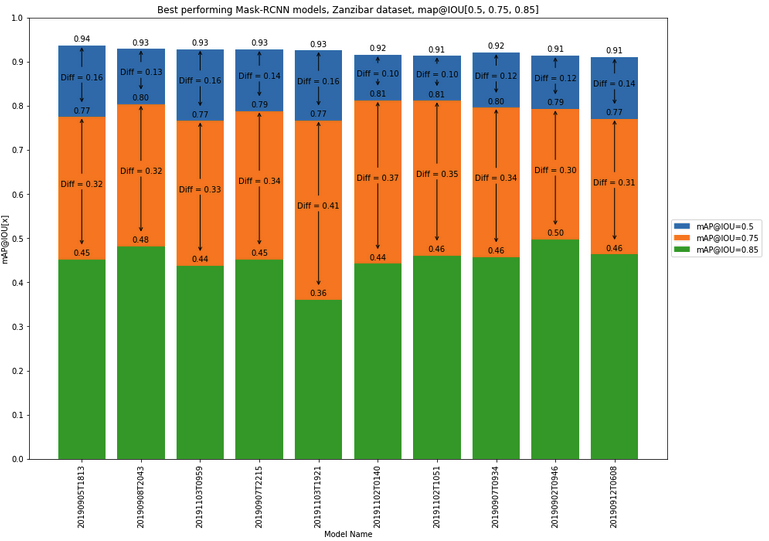
\includegraphics[scale=0.55]{Chapter3/figs/mask-RCNN-model-bar-chart.png}
	\end{center}
	\caption{mAP@IOU[0.5, 0.75, 0.85] scores for the best performing Mask-RCNN models trained on the Zanzibar dataset. See Table \ref{tab:MaskRCNNHyperparamTuningGridSearch} for each model's hyperparameters.}
	\label{fig:mAP-best-models-bar-chart}
\end{figure}

When deciding on which model hyperparameters are best for the task of cetacean segmentation, it is important to find a model with a high mAP@IOU[0.85] score. As the model will be used to perform segmentation before fine-grained classification, it is important the model is capable of removing as much background from the input image as possible. Any background included in the segmentation may adversely effect the photo-id process. Using this as criteria, model 20190902T0946 was selected as the best performing model. The model achieves an mAP@IOU[0.85] score of 0.5, an excellent result given the difficulty of the segmentation task. The model also performs well at the other evaluation thresholds, achieving mAP@IOU[0.5, 0.75] scores of 0.91 and 0.79 respectively. These scores verify the model is capable of segmenting cetacean fins from background with as little noise being included in the segmentation mask as possible.

An interesting point to note here is that 20190902T0946 did not achieve the highest mAP@IOU[0.5, 0.75] scores. As previously mentioned, these thresholds are often the ones included in segmentation literature to evaluate model performance. If just these thresholds were used for model selection, 20190902T0946 would not have been chosen. This highlights the need to select models based on metrics which make sense for the task at hand. As the model is required to remove as much background noise as possible, using a high threshold for evaluation makes sense. Thresholds higher than 0.85 were not utilised due to the low performance of all models at this threshold, although 20190902T0946 also achieves one of the best mAP@IOU[0.9] score of 0.150. Only one model, 20191102T0615 achieves a better score at this threshold, 0.158, however this model achieves lower performance at the chosen evaluation thresholds of 0.5, 0.75, and 0.85.

\subsection{An Evaluation of Optimal Model Hyperparameters}\label{ch:cetDet,sec:ModelSelection,sub:OptimalHyperparameters}

As discussed in Section \ref{ch:cetDet,sec:ModelSelection,sub:ModelSelectionBasedOnGridSearch} a filtering of the trained Mask-RCNN models was performed to determine the best model hyperparameters for the task of cetacean instance segmentation, with model 20190902T0946 ultimately being selected for future use. This model's hyperparameters, along with those of the other nine best performing models, can be seen in Table \ref{tab:best-mask-rcnn-models}.

\begin{table}[!ht]
	\tiny
	\begin{adjustbox}{width=\columnwidth, center}
		\begin{tabular}{cccccc}
			\toprule
			Model Name & Weight Decay &        RPN Anchor Scales & Optimiser & Augmentation Strategy & Pre-trained on MSCOCO? \\
			\midrule
				20190902T0946 &         0.01 &   (16, 32, 64, 128, 256) &      SGDR &                  aug1 &                  True \\
				20190905T1813 &        0.001 &  (32, 64, 128, 256, 512) &      SGDR &                  aug1 &                  True \\
				20190907T0934 &         0.01 &  (32, 64, 128, 256, 512) &      SGDR &                  None &                  True \\
				20190907T2215 &        0.001 &   (16, 32, 64, 128, 256) &      SGDR &                  aug2 &                  True \\
				20190908T2043 &       0.0001 &  (32, 64, 128, 256, 512) &      SGDR &                  aug1 &                  True \\
				20190912T0608 &       0.0001 &   (16, 32, 64, 128, 256) &      SGDR &                  aug1 &                  True \\
				20191102T0140 &         0.01 &  (32, 64, 128, 256, 512) &      SGDR &                  aug1 &                  True \\
				20191102T1051 &       0.0001 &   (16, 32, 64, 128, 256) &      SGDR &                  None &                  True \\
				20191103T0959 &         0.01 &  (32, 64, 128, 256, 512) &      SGDR &                  aug2 &                  True \\
				20191103T1921 &       0.0001 &   (16, 32, 64, 128, 256) &      SGDR &                  aug2 &                  True \\
			\bottomrule
		\end{tabular}
	\end{adjustbox}
	\caption{Hyperparameters of the best performing Mask-RCNN models on the Zanzibar dataset. Subset of Table \ref{tab:MaskRCNNHyperparamTuningGridSearch}.}
	\label{tab:best-mask-rcnn-models}
\end{table}

The hyperparameters of the best performing models provide an interesting insight into the training process. All ten of the models were trained using SGDR. This is interesting, as the current trend in deep learning network training is to utilise Adam \cite{karpathy_peek_2017}. Furthermore each model trained utilised transfer learning, with each model's parameters being initialised from a trained MSCOCO model provided by the model zoo. This highlights the need to utilise pre-trained models, especially cases where relativity small amounts of data are available to train a model from scratch. 

Half of the best models utilise the \textit{aug1} data augmentation strategy, defined in Section \ref{ch:cetDet,sec:initialTesting,sub:dataaugmentation}. The smallest RPN Anchor Scale, (8, 16, 32, 64, 128), has not been utilised by any of the best models, and the value of the weight decay hyperparameter is split between the three possible values. These splits highlight the need for a robust and in-depth hyperparameter search, as with the majority of hyperparameters searched no clear trend can be identified.

\subsection{Limitations of the Model}\label{ch:cetDet,sec:ModelSelection,sub:LimitationsOfBest}

As with any neural network trained on real world data, the best performing model, 20190902T0946, is not perfect. As can be seen through the mAP scores in Figure \ref{fig:mAP-best-models-bar-chart}, the model still fails to correctly detect in some instances. This section examines under what conditions 20190902T0946 fails for the purposes of model transparency. 

Sometimes there are instances where the detection fails to capture all of the individual. This seems to occur when parts of the animal are poorly lit or void of unique markings leading to a consistent matt dark colour scheme. An example of this behaviour can be seen in Figure \ref{fig:model-fail-bad-detection-and-split-individual}'s green detection. Here, the model has correctly detected the part of the animal's body which is above the waterline, but has failed to fully detect the matt dark dorsal fin. This poor detection may also be influenced by the undetected individual close behind the detected animal. 

Figure \ref{fig:model-fail-bad-detection-and-split-individual} also shows another good example of environmental conditions which cause the model to fail to correctly detect an individual. Due to wave movement covering a part of the left animal's body, the model has split this individual into two separate detections.

\begin{figure}[h]
	\begin{center}
		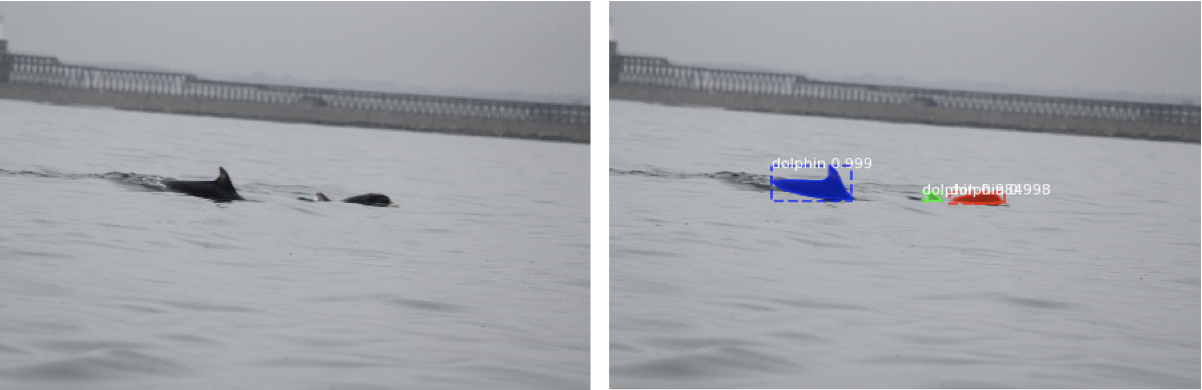
\includegraphics[scale=0.6]{Chapter3/figs/model-fail-split-individual.png}
	\end{center}
	\caption{Left: The input image passed to the cetacean detector. Right: The detection masks produced by the model overlaid onto the image. Note how the cetacean on the left has been split over two masks due to occlusion from a small wave.}
	\label{fig:model-fail-bad-detection-and-split-individual}
\end{figure}
 
The model also struggles in cases where the image contains an animal under the waterline but due to the clarity of the water is partly visible in the image. In this case the model often detects the individual under the waterline. Due to these individuals not being useful for identification purposes however, they were not labelled in the dataset and thus are deemed to be misclassifications when evaluating the model. Figure \ref{fig:model-fail-underwater} shows an example of this issue occurring.

\begin{figure}[h]
	\begin{center}
		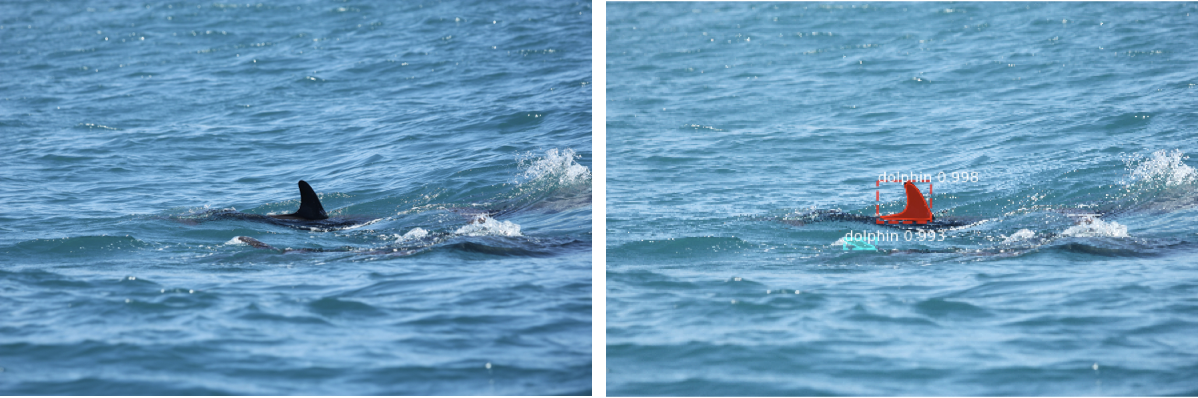
\includegraphics[scale=0.6]{Chapter3/figs/model-fail-underwater.png}
	\end{center}
	\caption{Left: The image passed to the cetacean detector. Right: The detection masks produced by the model overlaid onto the image. Note how the blue detection is of an individual under the waterline and only partly visible, and thus useless for identification purposes. }
	\label{fig:model-fail-underwater}
\end{figure}

The Zanzibar dataset contains a large number of images which contain other vessels as well as dolphins. This is due to the large marine eco-tourism industry within Zanzibar \cite{sharpe_indian_2019-1, berggren_sustainable_2007}. Whilst this issue may not be present in other survey areas where this model may be deployed, it still denotes an example of the model failing. In this case often parts of the boat, or a combination of the boat and the humans on the boat, may cause the model to incorrectly identify a grouping of pixels as a dolphin. An example of this can be seen in Figure \ref{fig:model-fail-boat}.
 
\begin{figure}[h]
	\begin{center}
		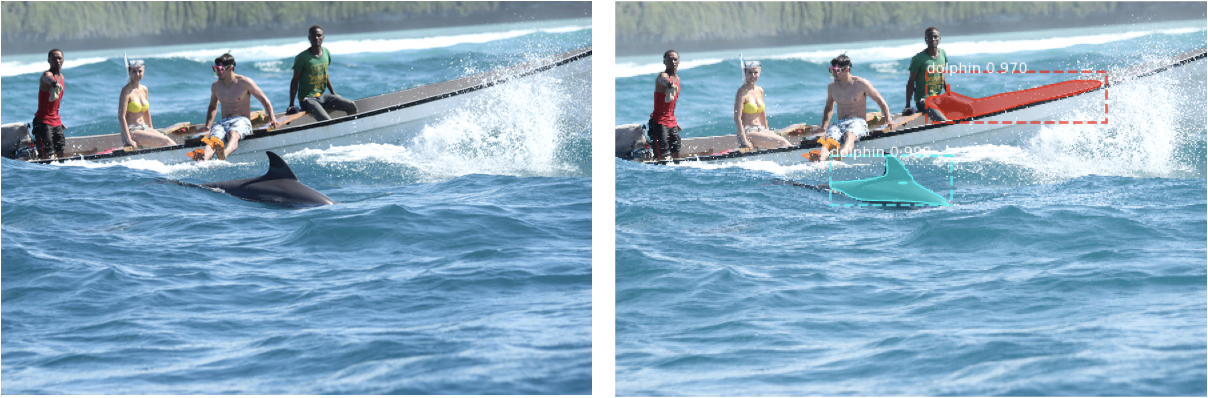
\includegraphics[scale=0.6]{Chapter3/figs/model-fail-boat.png}
	\end{center}
	\caption{Left: The image passed to the cetacean detector. Right: The detection masks produced by the model overlaid onto the image. Note how the red detection is a misclassification. The model believes a section of the boat's hull and the leg of the human to be a dolphin.}
	\label{fig:model-fail-boat}
\end{figure}

All of these mis-detections have an impact of the overall evaluation score of the model. These mis-detections will then be passed further down the system pipeline to be classified as individuals. To reduce the chances of this happening, a robust post-processing technique was developed.

\section{Mask Post-Processing Techniques}\label{ch:cetDet,sec:postProcessing}

At this stage, the system is capable of detecting cetaceans at an individual pixel level. Before these detections can be passed to the identification module, some post-processing of the output must be performed to allow for both a reduction in the computational expense of operating on the detector's output as well as ensuring that no potentially important information which will assist in an identification is lost. 

\subsection{Handling Multiple Detections}\label{ch:cetDet,sec:postProcessing,sub:handlingMultipleDetections}

When an image is ran through the Mask-RCNN detector, the number of outputs can vary depending on how many detected objects have a confidence score higher than 90\% (as discussed in Section \ref{ch:cetDet,sec:ModelSelection,sub:DetectionHyperparameters}). If no detections reach this threshold the image is discarded from further processing. This can occur if, for example, an image is taken by accident capturing the vessel's floor. If a single detection reaches the threshold, the resultant mask is passed downstream. 

Thanks to the tendency for cetaceans to travel in pods however, it is unlikely an image will contain only a single \texttt{dolphin} detection. In these situations the Mask-RCNN will output multiple detection masks, one per object. To handle this, the first stage of the post-processing methodology is to separate multiple detections for a single image. This ensures each \texttt{dolphin} detection is handled independently, mitigating the potential for an identification to be influenced by the others. An example of this behaviour can be seen in Figure \ref{fig:190730-001-MOLS0360_-detections}. Here, an image inputted to the Mask-RCNN detector has produced three detections which are above the threshold. As such, they have been split into three output masks for individual processing. Note that the first detected masks, visualised with a blue overlay on the input image, has been incorrectly detected as \texttt{dolphin} with a high confidence resulting in a binary mask. Further post-processing must be capable of handling background which has been incorrectly labelled, removing it before individual identification occurs.

\begin{figure}
	\begin{center}
		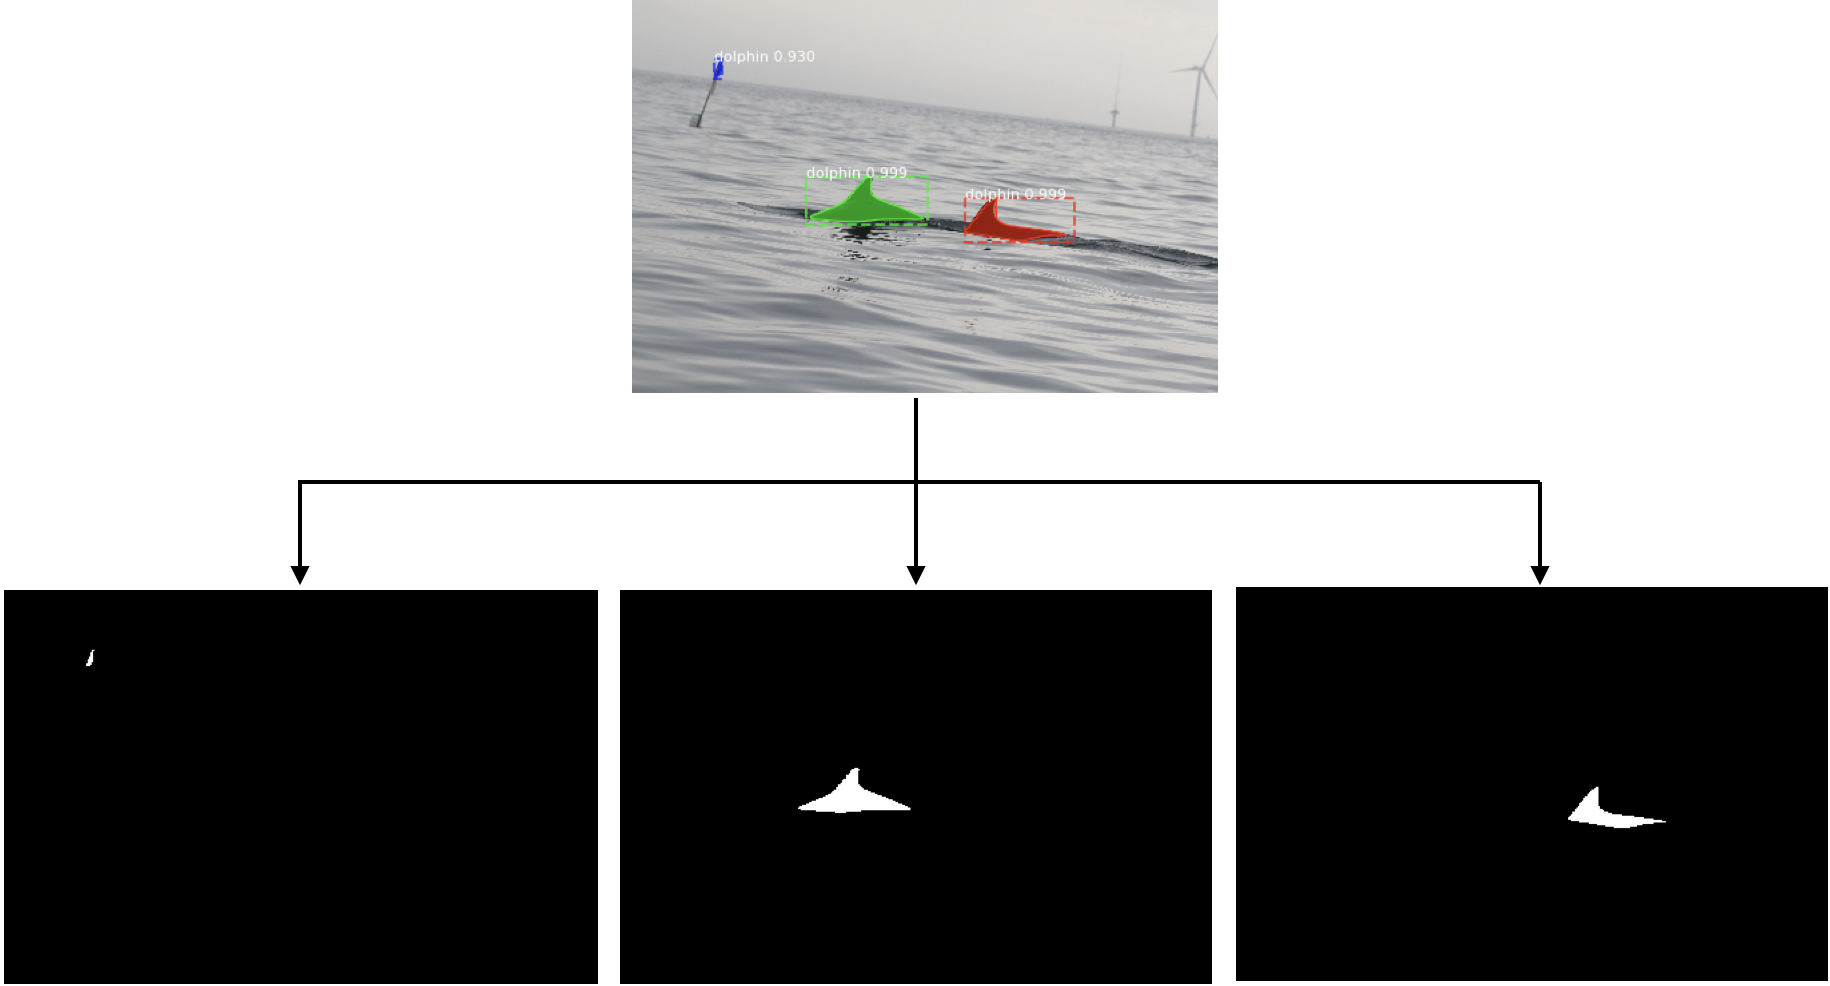
\includegraphics[scale=0.45]{Chapter3/figs/190730-001-MOLS0360_-detections.png}
	\end{center}
	\caption{A visualisation of the three \texttt{dolphin} detections for an input image produced by the Mask-RCNN detector. The detections are highlighted by the blue, green, and red overlays on the input image, top. The resultant detection masks once split are shown bottom, where a \texttt{dolphin} object is displayed in white.}
	\label{fig:190730-001-MOLS0360_-detections}
\end{figure}


\subsection{Morphological Transformations}\label{ch:cetDet,sec:postProcessing,sub:morphologicalTransformations}

In some situations a detected mask may contain an area of background inside the detection. This can be thought of as a hole in the detection, as seen in Figure \ref{fig:before-and-after-morphing-masks-only} (Left). Using \textit{a priori} knowledge of cetaceans, which would rarely if ever be captured with a hole, it can be deduced that a hole in the detection is highly unlikely and may cause a loss of useful identifying information. As such, any holes which are present in the masks must be filled.  

\begin{figure}
	\begin{center}
		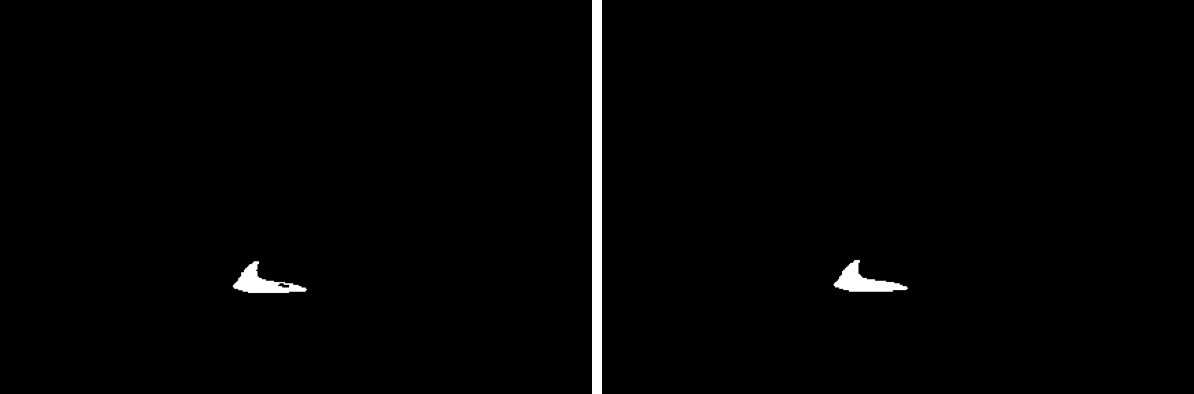
\includegraphics[scale=0.5]{Chapter3/figs/before-and-after-morphing-masks-only.png}
	\end{center}
	\caption{Left: A detection mask before closing has been applied. The detected \texttt{dolphin} object is displayed in white. Note the cluster of black background pixels inside. Right: The same detection mask after closing. Note the pixels which make up the hole have been converted to \texttt{dolphin}.}
	\label{fig:before-and-after-morphing-masks-only}
\end{figure}

This is achieved using morphological transformations, a set of operations which allow for the automated manipulation of the internal structure of binary images such as masks. The two fundamental morphological transformations are \textit{erosion}, which erodes away the boundaries of the masked object, and \textit{dilation}, which increases the size of the object by pushing the boundary out into the background space. These two operations can be utilised in various combinations to perform more complex transformations.

In order to remove a cluster of background pixels inside of a detection, each mask is \textit{closed} - dilated then eroded. This has the effect of removing any holes present inside the mask, as can be seen in Figure \ref{fig:before-and-after-morphing-masks-only} (Right). If no holes exist, the operation is still performed however the mask remains unchanged. By performing closing, the system ensures that no potentially identifiable information is lost as a result of an incomplete detection. 

\subsection{Background Subtraction}\label{ch:cetDet,sec:postProcessing,sub:bgExtraction}

Now that the masks have been cleaned using morphological transformations, it is possible to utilise them to perform background subtraction. This is an extremely important step in producing an accurate individual classification based on the detected \texttt{dolphin} object by ensuring a minimal amount of background noise is passed to the identification system.

As both the input image and resultant mask can be represented as matrices, these can be manipulated utilising a \textit{bitwise and} operation such that if pixel$_{i, j}$ in the input image is denoted as background in the mask, the values of pixel$_{i, j}$ can be set to [255, 255, 255] (white). This has the effect of whiting out any pixels not detected as part of the \texttt{dolphin} in the input, whilst keeping the pixels detected as \texttt{dolphin} intact.

An example of background subtraction utilising cleaned masks can be seen in Figure \ref{fig:190730-001-MOLS0360_-bg-subtraction}. Using the same input image as in Figure \ref{fig:190730-001-MOLS0360_-detections}, it can be seen that the \textit{bitwise and} operation whites all pixels in the image except those which have been classified as \texttt{dolphin} for each of the three output masks. Note at this point that the erroneous classification still remains. 

\begin{figure}
	\begin{center}
		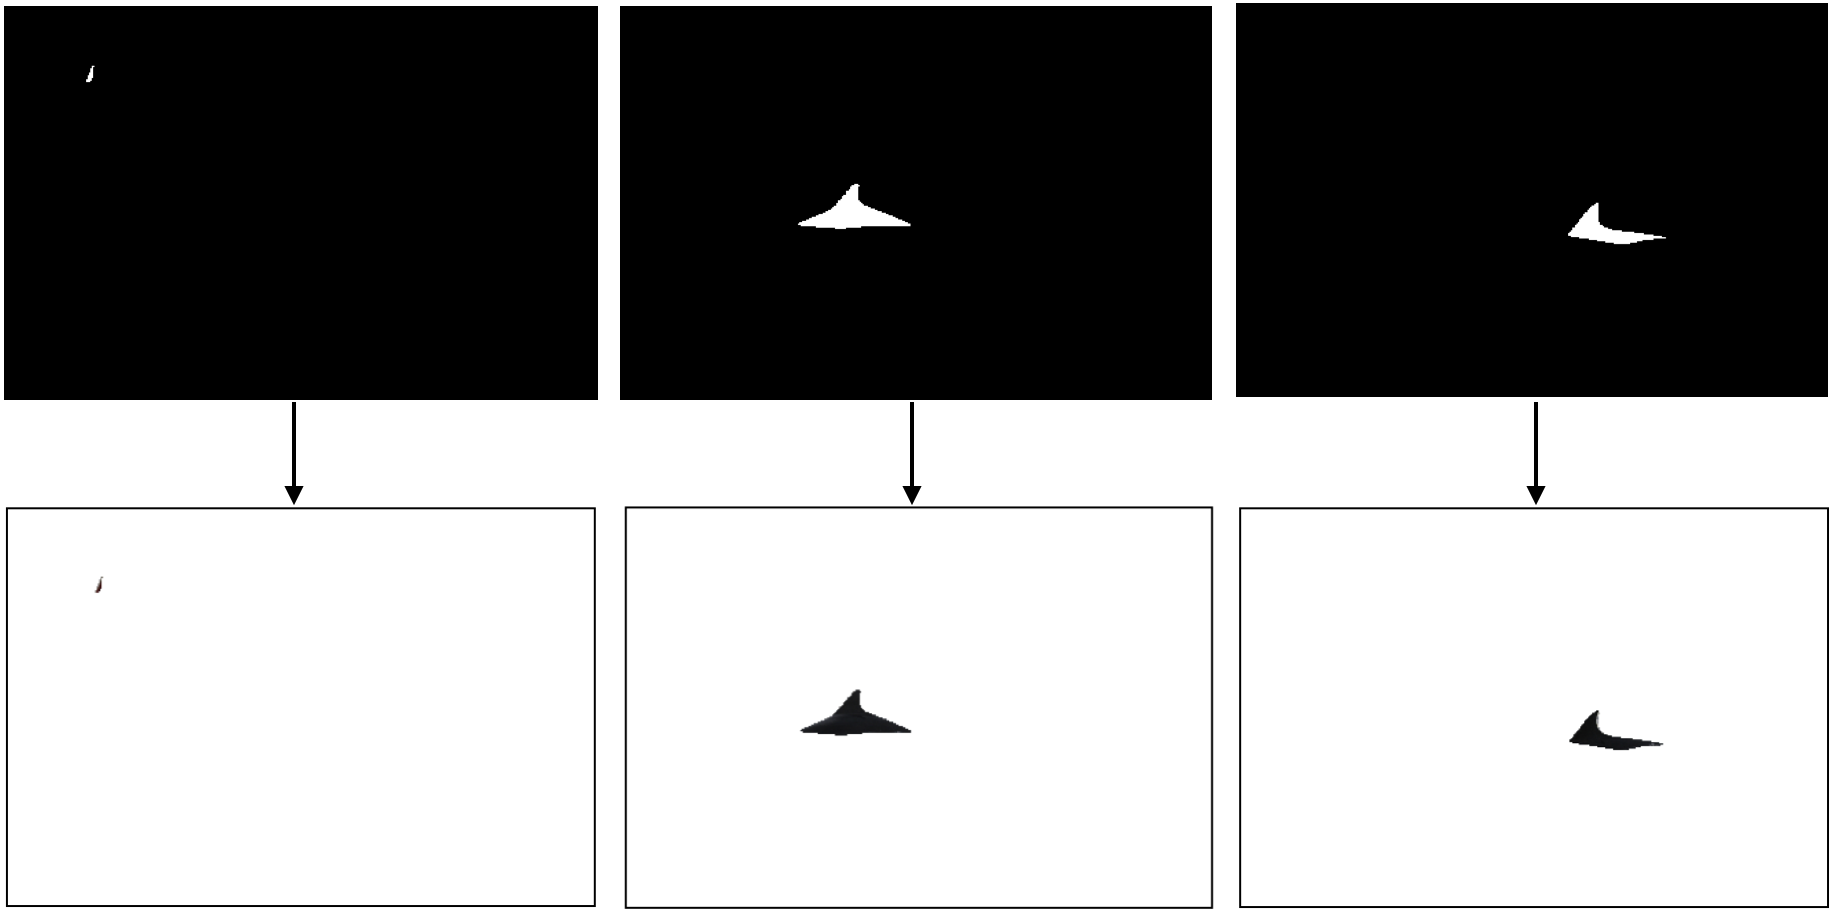
\includegraphics[scale=0.45]{Chapter3/figs/190730-001-MOLS0360_-bg-subtraction.png}
	\end{center}
	\caption{A visualisation of the three \texttt{dolphin} detections from Figure \ref{fig:190730-001-MOLS0360_-detections} before and after background subtraction.A border has been added to the background subtracted images for clarity.}
	\label{fig:190730-001-MOLS0360_-bg-subtraction}
\end{figure}

Whilst the background subtraction aims to reduce noise passed downstream to the individual identification module, it will not be possible to remove all noise. It may be the case, such as in Figure \ref{fig:fin-extraction-unclean}, that some background pixels have been mislabelled as \texttt{dolphin} and are connected to at the edges of the object. As a result, morphological transformation and background subtraction are unable to remove the mislabelled pixels. This may affect the accuracy of identification downstream unless the system is robust enough to deal with this.

\begin{figure}
	\begin{center}
		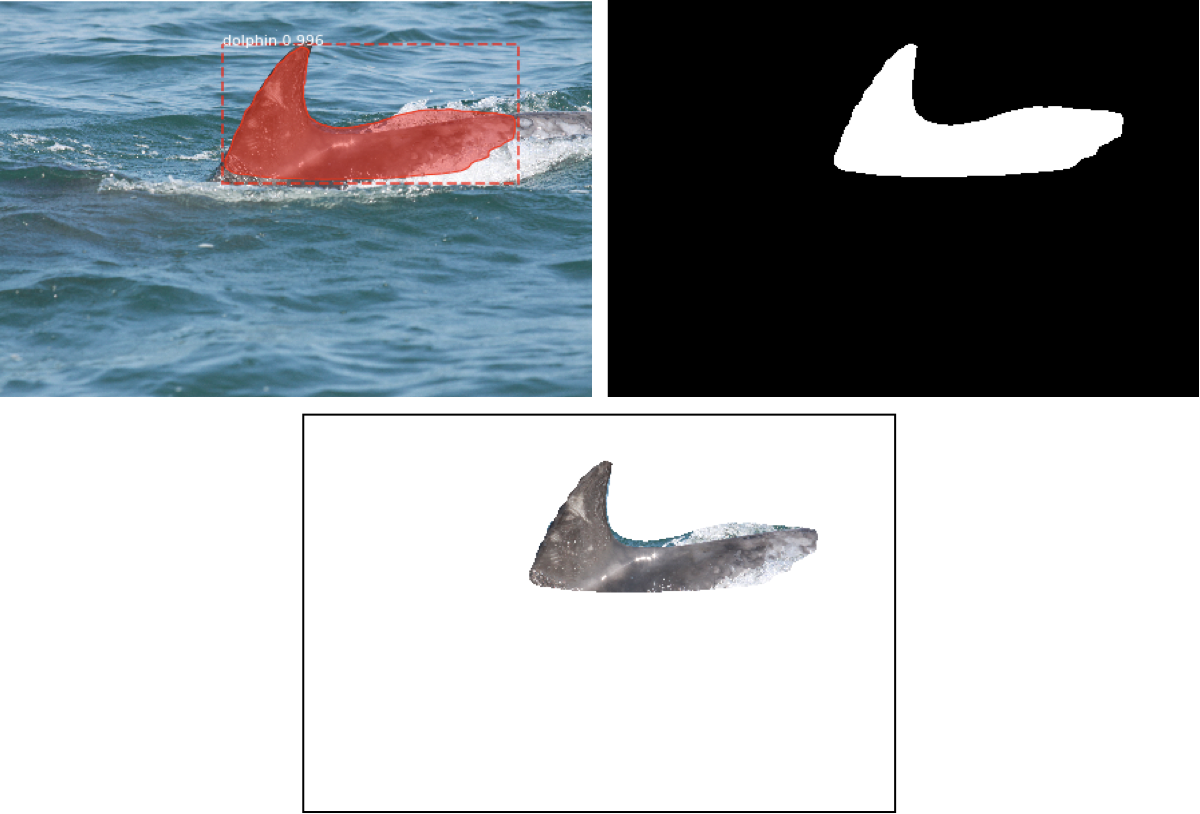
\includegraphics[scale=0.5]{Chapter3/figs/fin-extraction-unclean-uncropped.png}
	\end{center}
	\caption{Top Left: A visualisation of the \texttt{dolphin} detection for an input image produced by the Mask-RCNN detector, alongside the confidence score. The detector has incorrectly labelled some pixels as \texttt{dolphin}. Top Right: The resultant detection mask after morphological transformation. Bottom: The resultant output image after \textit{bitwise and} operations performed between the input image and the cleaned detection mask. Note the mislabelled pixels are present after cleaning and background subtraction. A border has been added for clarity.}
	\label{fig:fin-extraction-unclean}
\end{figure}

\subsection{Colour Thresholding Mask Components}\label{ch:cetDet,sec:postProcessing,sub:colourThresholdingMaskComponents}

In some cases a single detection mask may consist of multiple components. This may occur if, for example, an area of splash has been erroneously included as part of a detection. As cetaceans cannot be made up of multiple disjoint components, it is known that some of these must be noise and can be removed. 

The outer layer of a cetacean's skin is often a consistent grey colouring. This information can be utilised to filter out noisy components of the mask during post-processing. By comparing the colour composition of each detected object against a calculated \textit{dolphin-like} threshold, it is possible to discard mask components which have been erroneously detected.

In order to be able to compare each mask component's composition against a \textit{dolphin-like} colour threshold, the values of the threshold must first be determined. To achieve this, each image in the Zanzibar dataset was ran through the Mask-RCNN detector. Histograms of the three RGB colour channel pixel intensities for each object classification (\texttt{dolphin} or background) were recorded, giving a total of six histograms per image. 

Once complete the histogram groups were combined to give six global pixel intensity distributions, which can be seen in Figure \ref{fig:global-histogram}. From the charts it can be seen that, regardless of colour channel, there is a near inversion in the distribution of pixel intensities between those detected as \texttt{dolphin} and those not, strongly suggesting it is possible to determine if a component is erroneous based on its colour composition.

\begin{figure}
	\begin{center}
		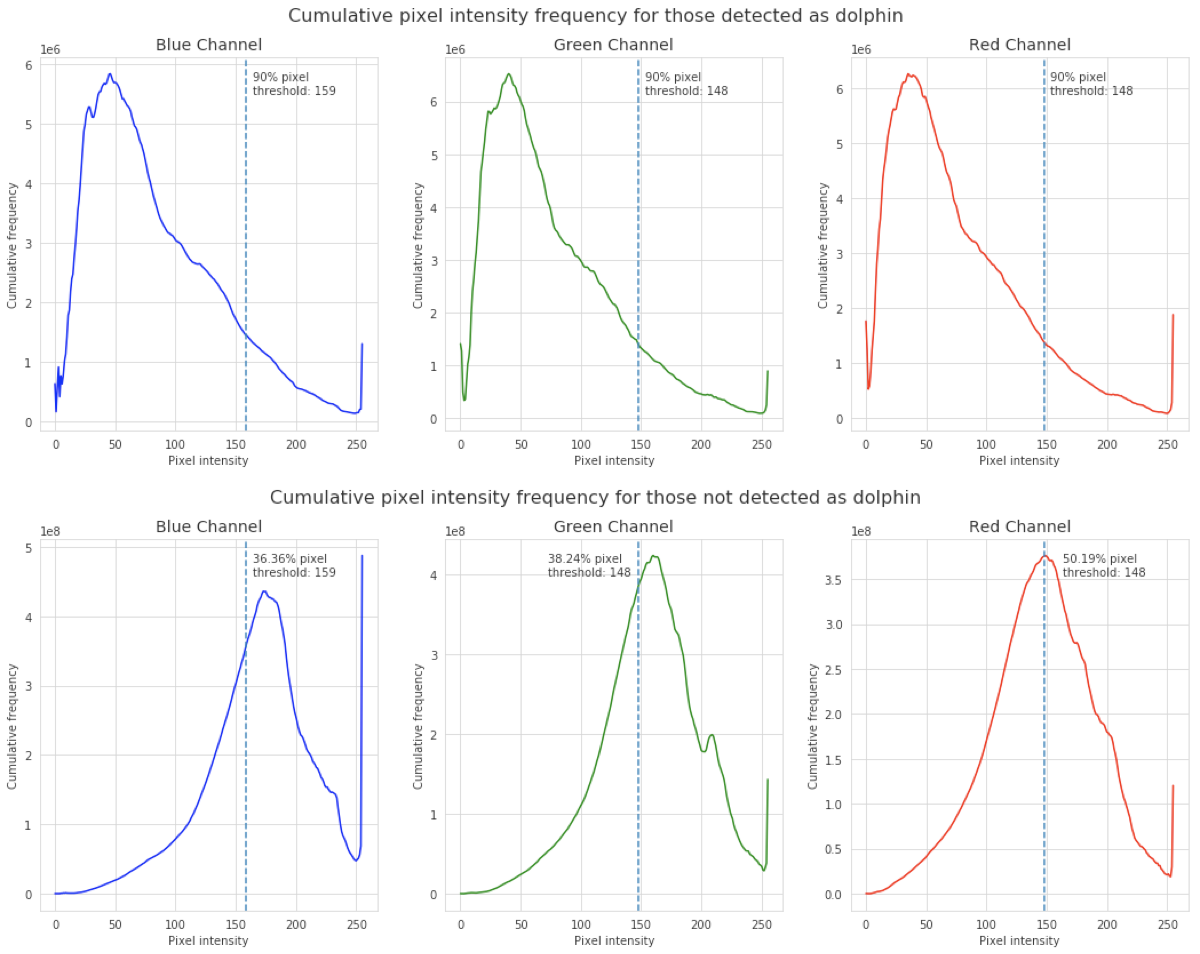
\includegraphics[scale=0.7]{Chapter3/figs/histogram.png}
	\end{center}
	\caption{The global range of pixel intensities for each RGB colour channel, split by pixel classification.}\label{fig:global-histogram}
\end{figure}

Using the global distribution histograms, a \textit{dolphin-like} threshold was determined. For all masks detected as \texttt{dolphin}, 90\% of the RGB pixel intensities are below [148, 148, 159]. The colour representing this threshold can be seen in Figure \ref{fig:colour-threshold}. In contrast only 50.19\%, 38.24\%, and 36.36\% of the background pixels for each RGB channel respectively are below this threshold. As noise components in the mask are often areas of water or splash, these components will be likely much lighter in composition than cetaceans, and thus can be removed from the mask with confidence. An example of colour thresholding removing noise from a mask can be seen in Figure \ref{fig:190827-001-MOLS0078_-colour-thresholding-splash-removed}.

\begin{figure}
	\begin{center}
		
\includegraphics[scale=0.3]{Chapter3/figs/148-148-159.png}
	\end{center}
	\caption{A representation of the RGB threshold for \textit{dolphin-like}, colour [148, 148, 159]. In the Zanzibar dataset, 90\% of pixels detected as \texttt{dolphin} have intensities below this threshold.}\label{fig:colour-threshold}
\end{figure}

\begin{figure}
	\begin{center}
		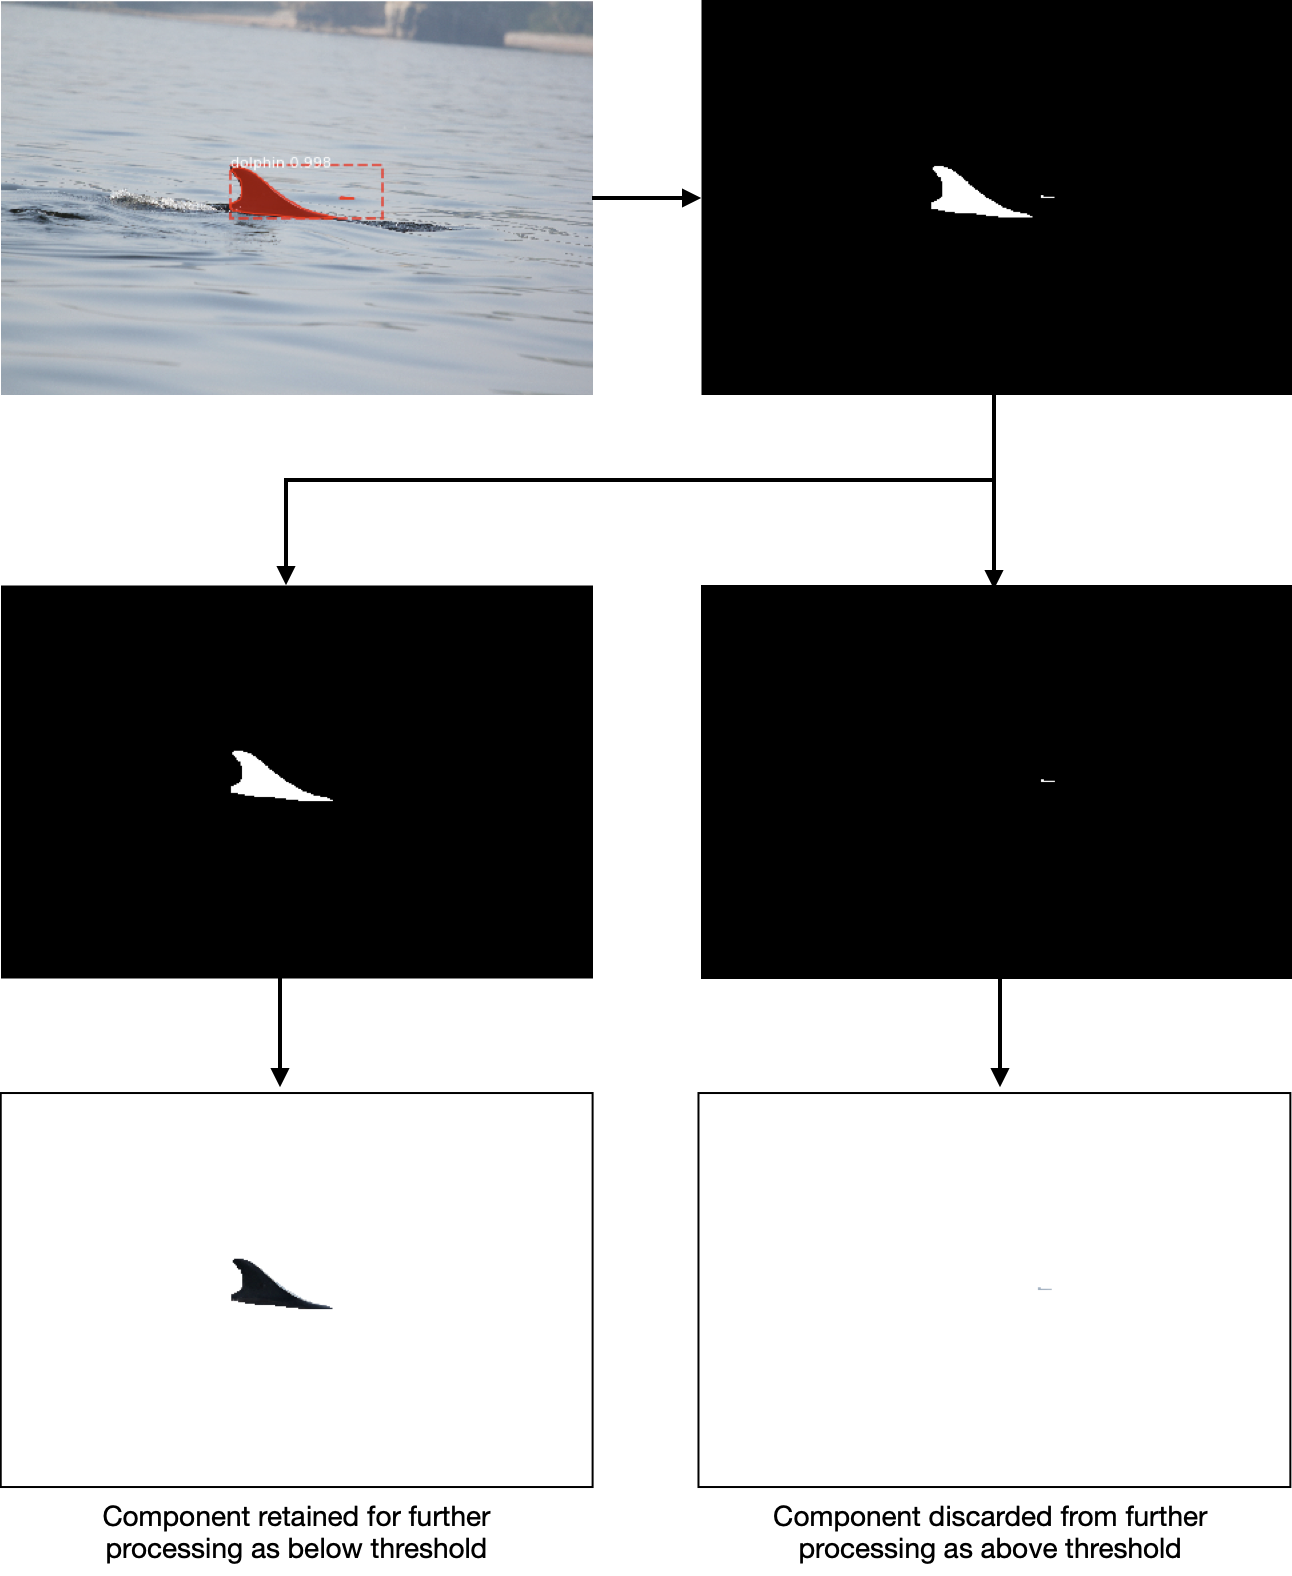
\includegraphics[scale=0.5]{Chapter3/figs/190827-001-MOLS0078_-colour-thresholding-splash-removed.png}
	\end{center}
	\caption{Workflow detailing colour thresholding to remove an area of disjoint splash which has been detected as part of a \texttt{dolphin} object. The detection mask is split into each component. The resultant background subtracted images are then colour thresholded. As a result, the erroneous splash is discarded. }\label{fig:190827-001-MOLS0078_-colour-thresholding-splash-removed}
\end{figure}

During testing however it was found that when checking detections at an individual image level rather than globally, considering a mask component to be \textit{dolphin-like} if 90\% of the pixels were below the colour threshold was too restrictive. Utilising such a high percentage bar sometimes rejected valid detections which may have been over-exposed due to lighting conditions. As such, whilst the colour threshold was kept the same, it was found that reducing the percentage check to 50\% provided enough leeway such that over-exposed but valid detections were kept whilst still rejecting a large portion of erroneous ones. Figure \ref{fig:190723-001-MOLS0752_-fin-removed-at-90-kept-at-50} shows an example detection which would be discarded if the 90\% global threshold was used per image, but is retained if this is dropped to a 50\% check.

\begin{figure}
	\begin{center}
		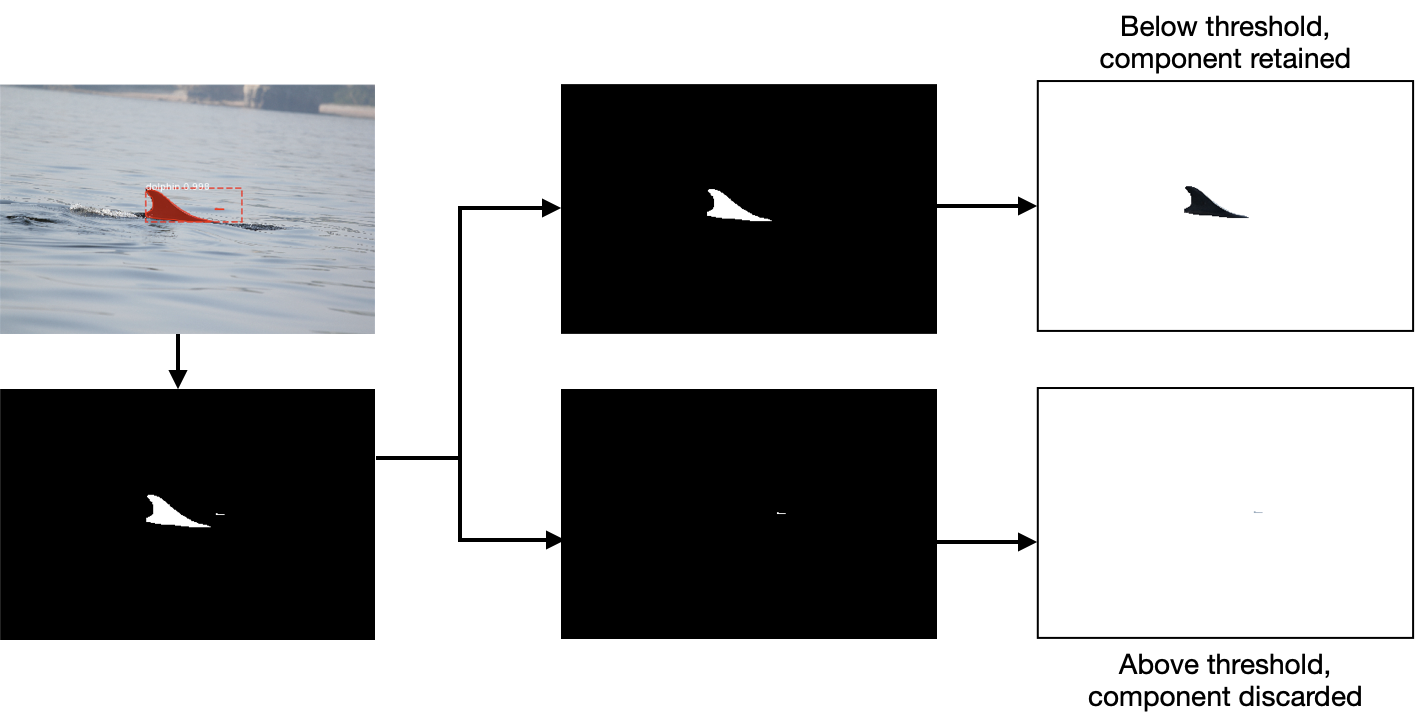
\includegraphics[scale=0.7]{Chapter3/figs/190723-001-MOLS0752_-fin-removed-at-90-kept-at-50.png}
	\end{center}
	\caption{Workflow showing how utilising the 90\% global threshold may lead to over-exposed detections being erroneously discarded. A \texttt{dolphin} object is detected whose mask consists of multiple components.  One of the components, which contains a valid area of detection, is shown in stage 3 of the workflow. Checking to see if 50\% of the pixels in the component are below the threshold retains the detection, whilst checking at 90\% discards it.}\label{fig:190723-001-MOLS0752_-fin-removed-at-90-kept-at-50}
\end{figure}

It may be the case that multiple components in an image meet the conditions set by the threshold to be kept. In this case, each component of the mask is split into its own image, in a similar process as outlined in Section \ref{ch:cetDet,sec:postProcessing,sub:handlingMultipleDetections}. If a mask only contains one component, then colour thresholding is not applied. This ensures no detections by the Mask-RCNN are completely ignored due to post-processing, preventing the discarding of a \texttt{dolphin} object mask which contains no disjoint components however is above the threshold, such as in the event of over-exposure. This condition also has the effect however of allowing fully erroneous detections to pass downstream, such as the flag detected in Figures \ref{fig:190730-001-MOLS0360_-detections} and \ref{fig:fin-extraction-unclean}. Any erroneous detections which pass downstream at this stage must now be handled by the identification module.

\subsection{Cropping}\label{ch:cetDet,sec:postProcessing,su:cropping}

At this point outputs from the Mask-RCNN detector have been post-processed to remove as much noise from the detected masks as possible, and these have been utilised to perform background subtraction. This results in an output image containing mostly white pixels surrounding a detected \texttt{dolphin} object. This image is the same size as the one inputted to the detector, which can often be many thousands of pixels, although the vast majority of these are now un-needed.

\begin{figure}
	\begin{center}
		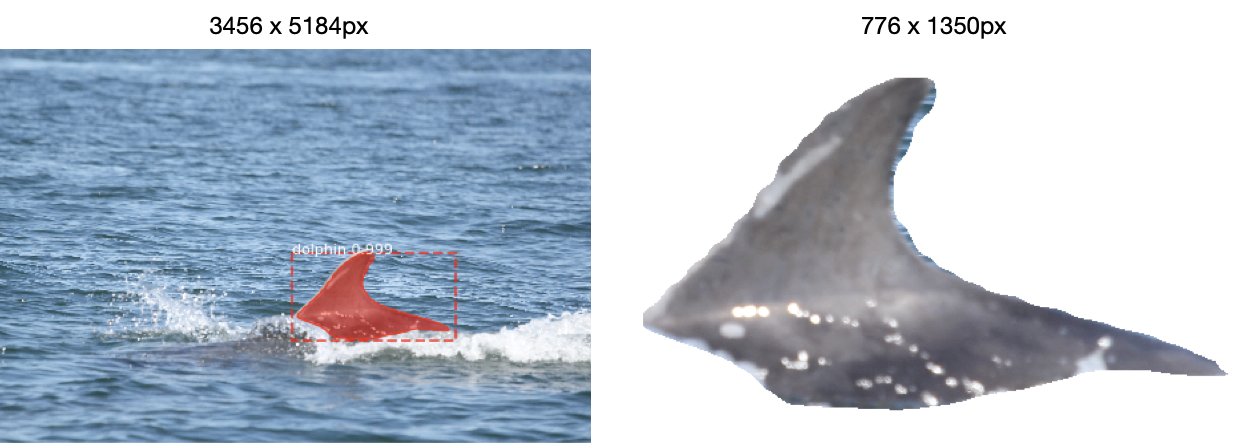
\includegraphics[scale=0.5]{Chapter3/figs/190627-001-MOLS0028_-crop.png}
	\end{center}
	\caption{Left: An input image and overlaid detection mask. Right: The corresponding cropped output image after post-processing. Original image sizes are displayed above each image. Images have been resized for clarity.}\label{fig:190627-001-MOLS0028_-crop}
\end{figure}

As a result, the images outputted from the background detector are now cropped down to contain just the object of interest. This has the effect of vastly reducing the image file size, which in turn reduces the computational expense of operating on them downstream. In Figure \ref{fig:190627-001-MOLS0028_-crop} for example, the input image to the detector is of size 3456x5184 pixels. After post-processing, the resulting output image is now of size 776x1350px, approximately a 94.2\% reduction in image size whilst still keeping identifying information,  such as the white pigmentation on the dorsal fin, present. This cropping also has the effect of centring the detected \texttt{dolphin} objects in the final output image. 


\section{Summary}\label{ch:cetDet,sec:Summary}

This Chapter discusses the project's need for a model capable of cetacean detection, both from a technical and environmental perspective. The key reasons behind the use of instance segmentation masks rather than the relatively less computational and time expensive bounding boxes is explained, with evidence showing how the difficulty of the task influenced this move. Once the system requirements and underlying model architecture have been identified, the Chapter then examines the use of model hyperparameter optimisation to train a model capable of cetacean detection via instance segmentation masks. The use of model pretraining is also explored, and highlights the benefits of this approach even when using a pretraining dataset who's domain and distribution are vastly different to the final model's goal. Finally, the Chapter examines the use of post-processing techniques to improve the output of the Mask-RCNN's detections for use in downstream tasks. 

The final result of this Chapter is a Mask-RCNN model capable of high mAP even at large IoU thresholds. The model's resulting detections are coupled with a post-processing pipeline capable of greatly reducing the amount, and improving the quality of, data which subcomponents further into the pipeline are required to operate on. This allows for greater computational efficiency downstream as well as ultimately more accurate and confident individual identifications.

It is of great importance that the trained Mask-RCNN model is capable of detecting cetaceans in photo-id data which has been gathered in different geospatial and temporal areas. It is also important that the detector is capable of similarly high levels of accuracy without re-training on data from that geographic area. Use of the detector on data collected in a different geospatial and temporal area, as well as the transformation of this data into a useable photo-identification dataset, is explored in Chapter \ref{ch:NDD}.


%%%%%%%%%%%%%%%%%%%
